\chapter{Justificación de diseño y mockups}\label{chap:diseno}
El \emph{dashboard} es uno de los tres componentes del sistema (junto al agente PEP local y la API PDP) y es el punto de interacción directa del administrador de seguridad con el motor de \emph{scoring} híbrido (Isolation Forest + LSTM Autoencoder). Su función no es cosmética: es la interfaz mediante la cual se cumplen CU-02 (ajuste de umbrales y políticas de respuesta) y se da visibilidad operativa a CU-01 (detección y mitigación automática).

El relevamiento cubre las 6 pantallas navegables del \emph{dashboard} (Usuarios, Con historial, Alertas, Umbrales, Auditoría y Estado del sistema), la pantalla de acceso (\emph{Login}) y la vista de detalle de usuario, a la que se llega haciendo clic sobre una fila del listado de Usuarios.

\section{Metodología de diseño}
El diseño de este \emph{dashboard} no parte de un \emph{wireframe} estático, sino que se construye de forma iterativa, validando cada pantalla contra los requerimientos funcionales que soporta (RF-12 a RF-17, RNF-07, RNF-15) y refinando la presentación visual. Esa distinción se documenta explícitamente para no sobrerrepresentar el proceso: lo que se muestra a continuación no es un registro histórico de bocetos previos a la implementación, sino una reconstrucción de \emph{wireframes} estructurales a partir de las pantallas ya construidas y validadas, que documenta la arquitectura de información y las decisiones de \emph{layout} de forma independiente del estilo visual final.

Cada \emph{wireframe} de este documento representa la estructura de esa pantalla ya validada (agrupación de información, jerarquía visual y controles disponibles). Se dibujan en formato de un \emph{wireframe} de baja-media fidelidad, sin el detalle de estilo final que sí se justifica por separado en la Sección~\ref{sec:decisiones-transversales-mockups} y que se puede contrastar directamente contra la pantalla real.

\section{Arquitectura de navegación}
Todas las pantallas comparten una barra superior fija con: el nombre del sistema, 6 accesos directos a las secciones (Usuarios, Con historial, Alertas, Umbrales, Auditoría, Estado del sistema), un indicador de alertas activas y un selector de tema claro/oscuro. Esta estructura común reduce la carga cognitiva del administrador al moverse entre las distintas vistas operativas: es la misma decisión de \emph{layout} en las 6 pantallas, solo cambia el contenido central.

\section{Catálogo de pantallas}
Para cada pantalla se presenta el \emph{wireframe} estructural de baja fidelidad, la captura real del \emph{frontend} implementado, y una tabla de justificación de diseño que ata cada decisión visual a un requerimiento funcional, no funcional o caso de uso concreto.

\subsection{Acceso (Login)}
Pantalla previa a cualquier vista operativa. Permite el acceso a la configuración del sistema (umbrales, acciones, notificaciones) mediante credencial de administrador, sin introducir roles nuevos ni afectar la autorización real de escritura de la API. El diseño es mínimo: una sola tarjeta centrada, sin distracciones, ya que su única función es autenticar antes de continuar. La Figura~\ref{fig:mockup-login-wireframe} presenta el \emph{wireframe} de la pantalla y la Figura~\ref{fig:mockup-login-real}, la pantalla implementada.

\begin{figure}[t]
	\centering
	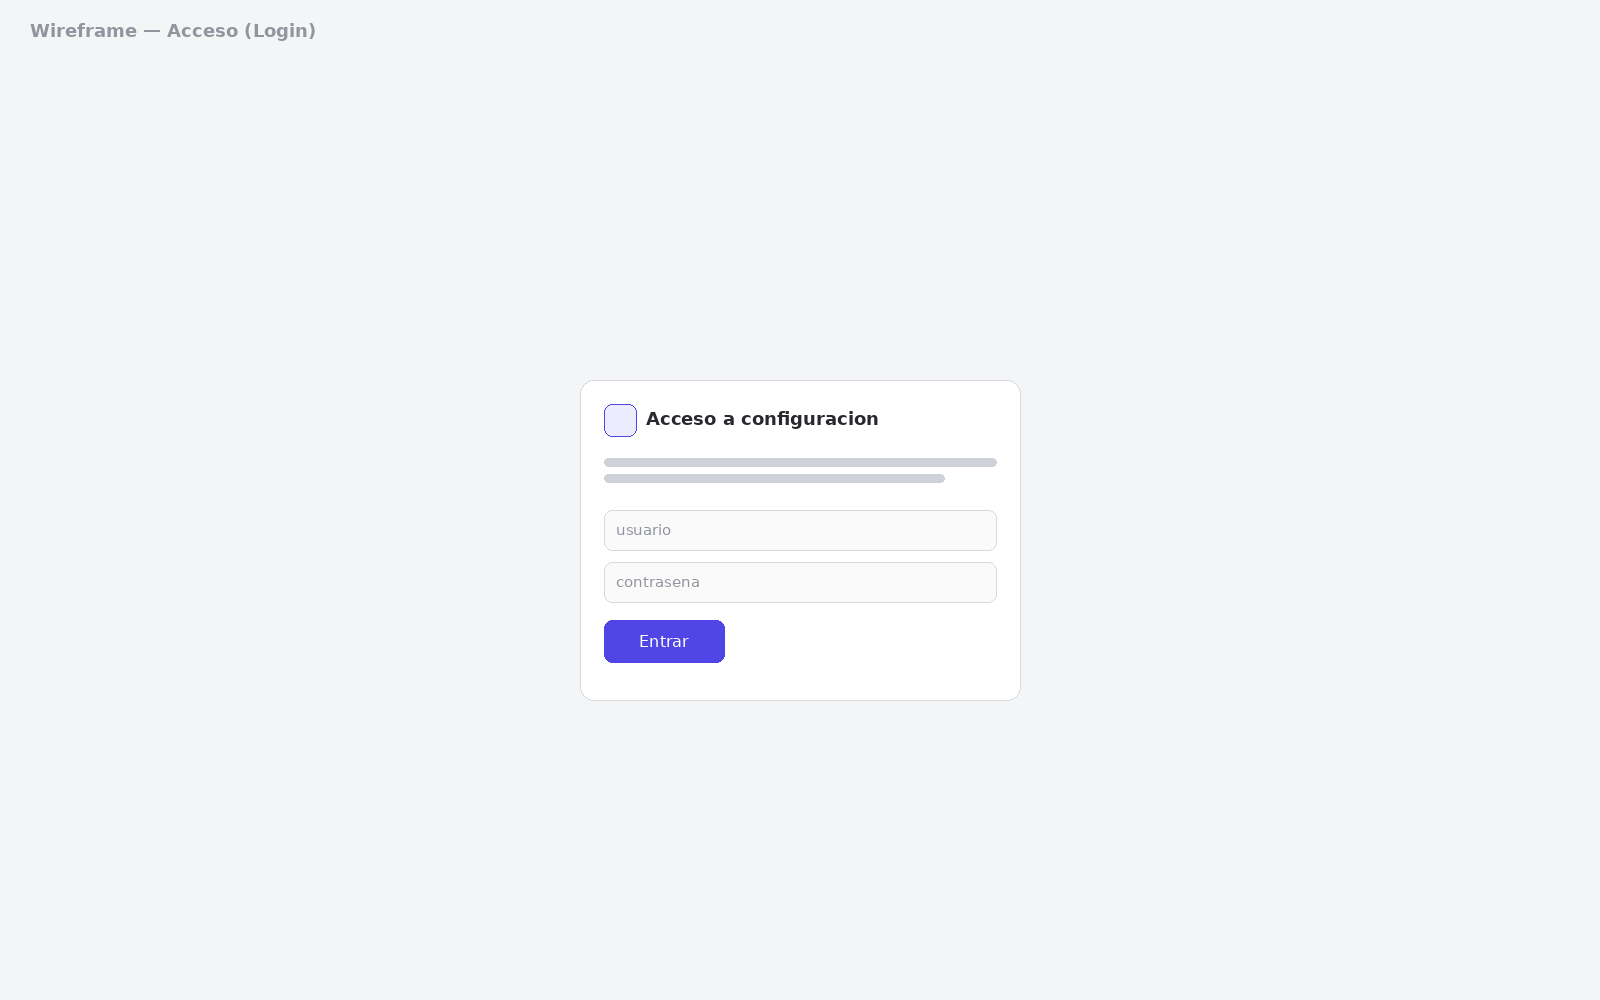
\includegraphics[width=0.8\textwidth]{images/mockups/mockup-login-wireframe.png}
	\caption{Wireframe de baja fidelidad: Acceso (Login)}
	\label{fig:mockup-login-wireframe}
	{\small Fuente: elaboración propia.\par}
	\bigskip
	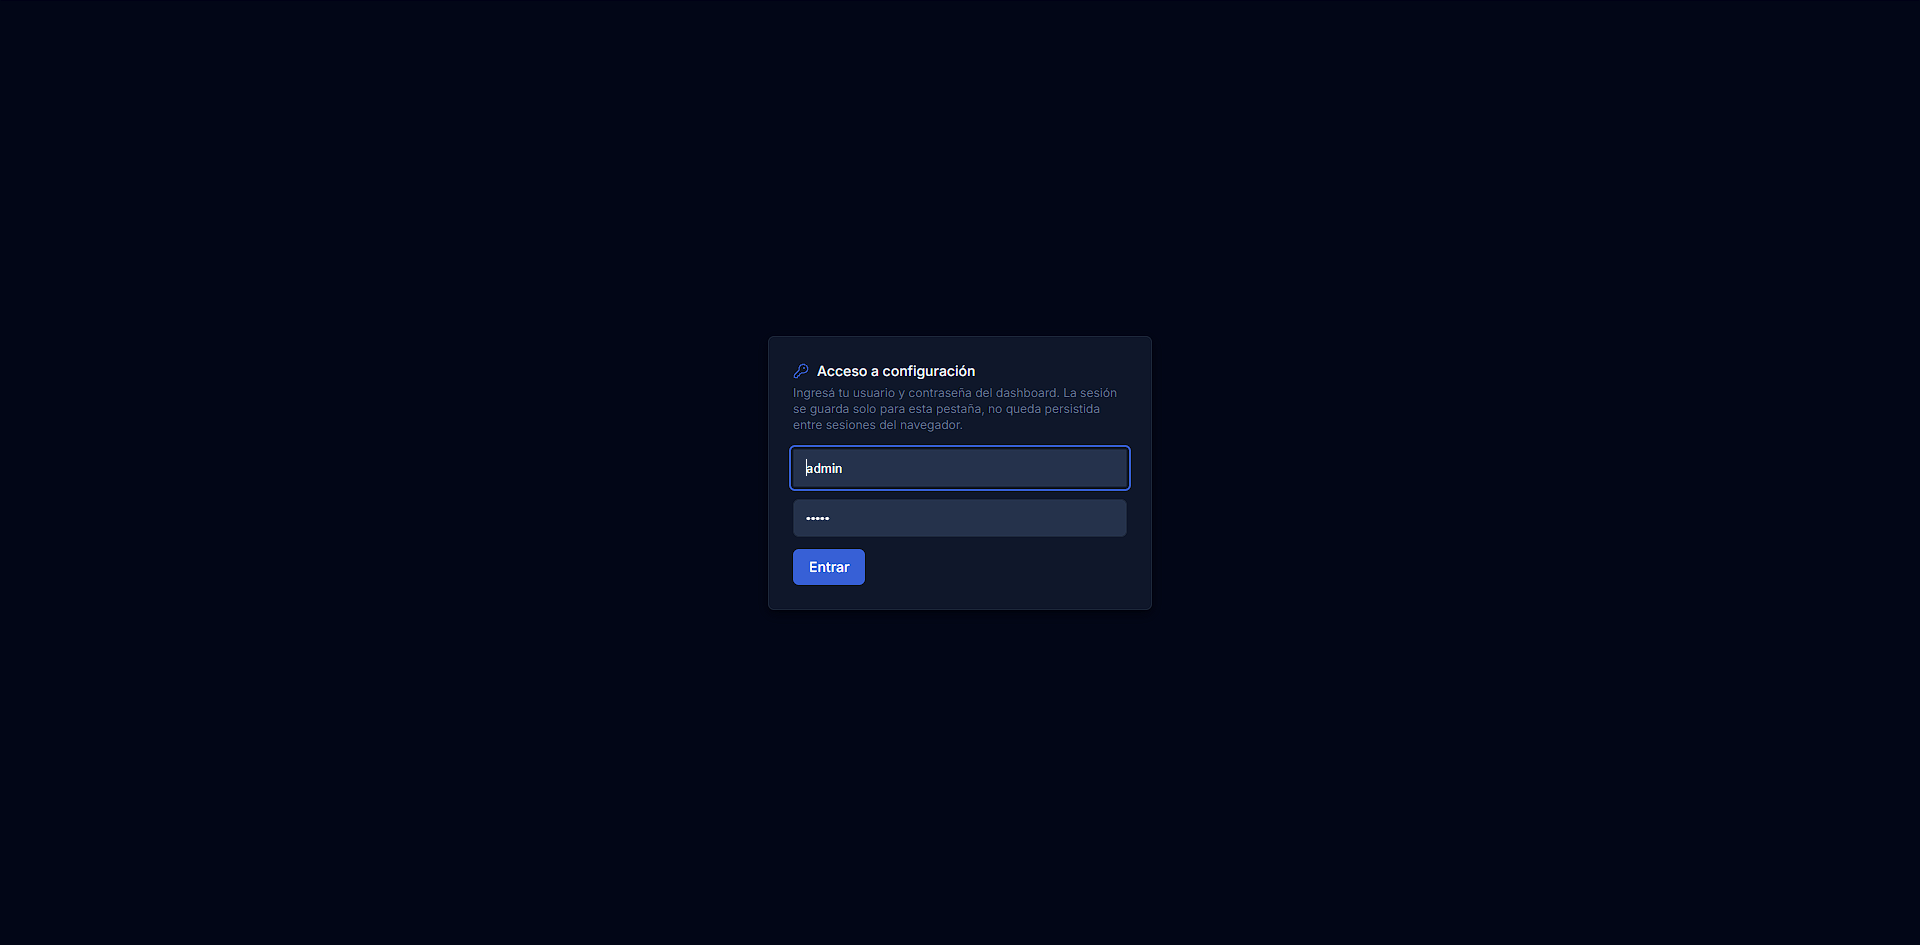
\includegraphics[width=0.8\textwidth]{images/mockups/mockup-login-real.png}
	\caption{Pantalla real: \texttt{/login}}
	\label{fig:mockup-login-real}
	{\small Fuente: elaboración propia, captura del sistema.\par}
\end{figure}
\FloatBarrier

\begin{longtable}{p{1.8cm}p{12.8cm}}
	\caption{Justificación de diseño: Acceso (Login)}
	\label{tab:mockup-login}\\
	\hline
	\textbf{ID} & \textbf{Justificación de diseño} \\
	\hline
	\endfirsthead
	\hline
	\textbf{ID} & \textbf{Justificación de diseño} \\
	\hline
	\endhead
	RNF-15 & El formulario centrado sobre fondo oscuro con un único punto de foco (usuario/contraseña/botón) prioriza claridad inmediata sobre densidad de información, no hay nada más que decidir en esta pantalla. \\
	\hline
	HU-14 / RNF-03 & Pantalla de inicio de sesión que restringe el acceso al \emph{dashboard}; la autorización efectiva de las operaciones de configuración la valida la API mediante la clave. \\
	\hline
	CU-02 & Es el punto de entrada obligatorio antes de que el administrador pueda ajustar umbrales o políticas de respuesta, cerrando el flujo descrito en el caso de uso. \\
	\hline
\end{longtable}
\FloatBarrier

\subsection{Usuarios (listado)}
Lista a todos los usuarios monitoreados con su nivel de riesgo actual, la acción de mitigación vigente, la cobertura del \emph{score} y su última actividad. Es la vista que responde directamente a RF-16: dar visibilidad en tiempo real al administrador antes de que tenga que entrar al detalle de cada usuario. La Figura~\ref{fig:mockup-usuarios-wireframe} presenta el \emph{wireframe} de la pantalla y la Figura~\ref{fig:mockup-usuarios-real}, la pantalla implementada.

\begin{figure}[t]
	\centering
	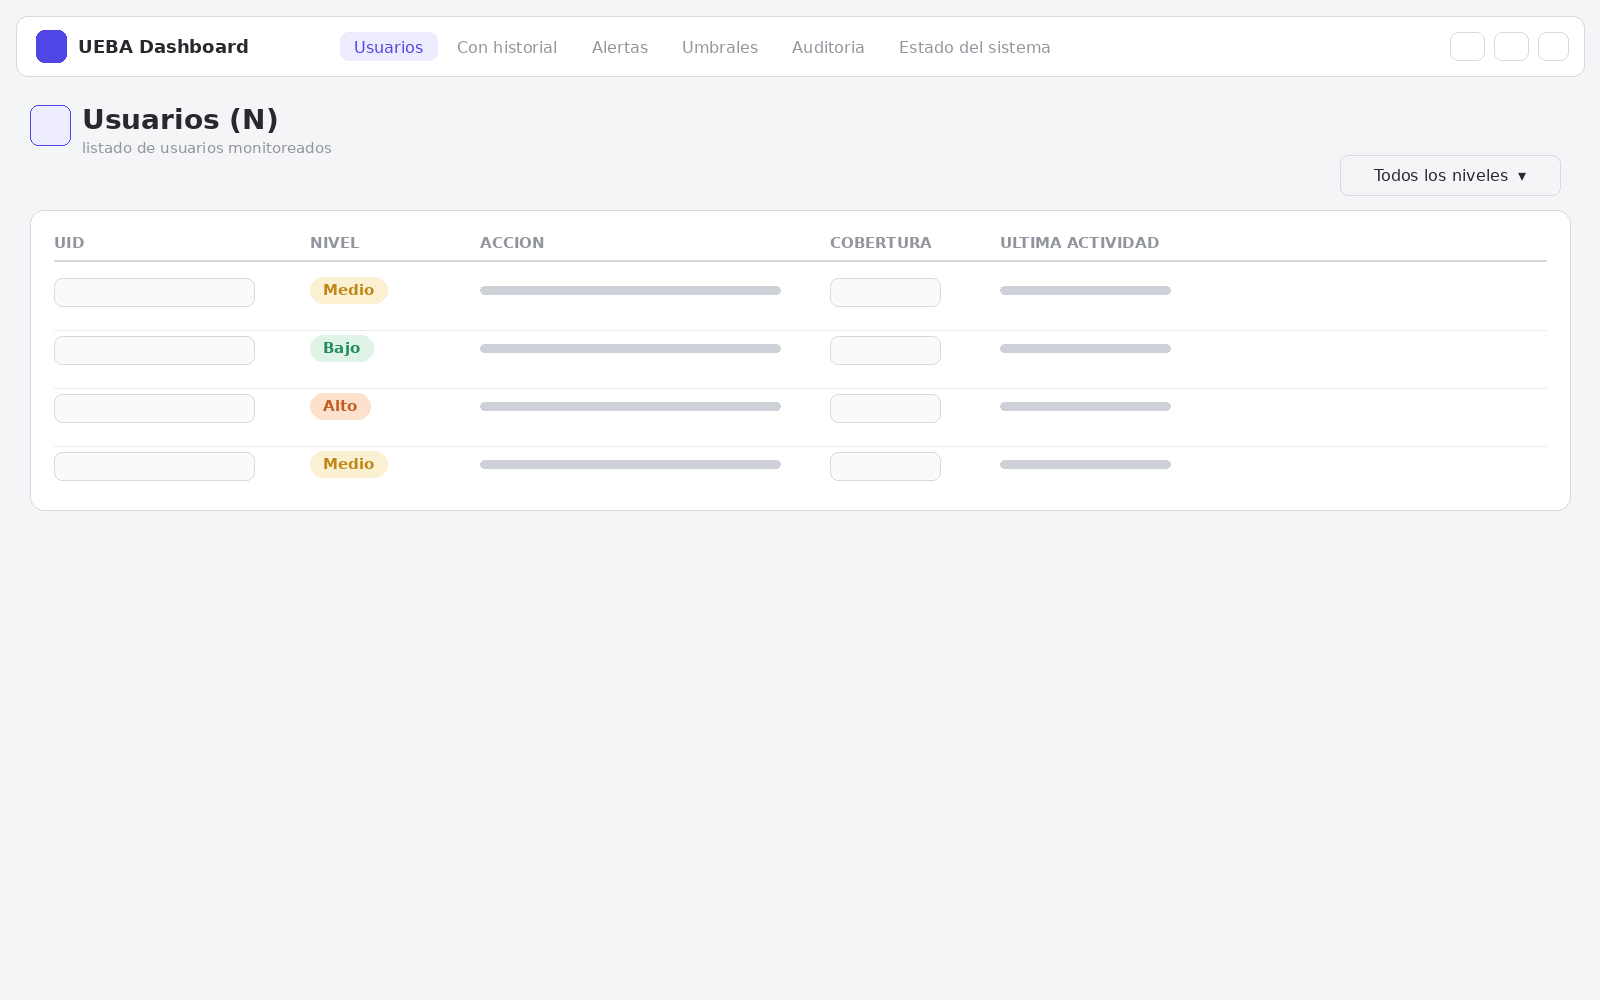
\includegraphics[width=0.8\textwidth]{images/mockups/mockup-usuarios-wireframe.png}
	\caption{Wireframe de baja fidelidad: Usuarios (listado)}
	\label{fig:mockup-usuarios-wireframe}
	{\small Fuente: elaboración propia.\par}
	\bigskip
	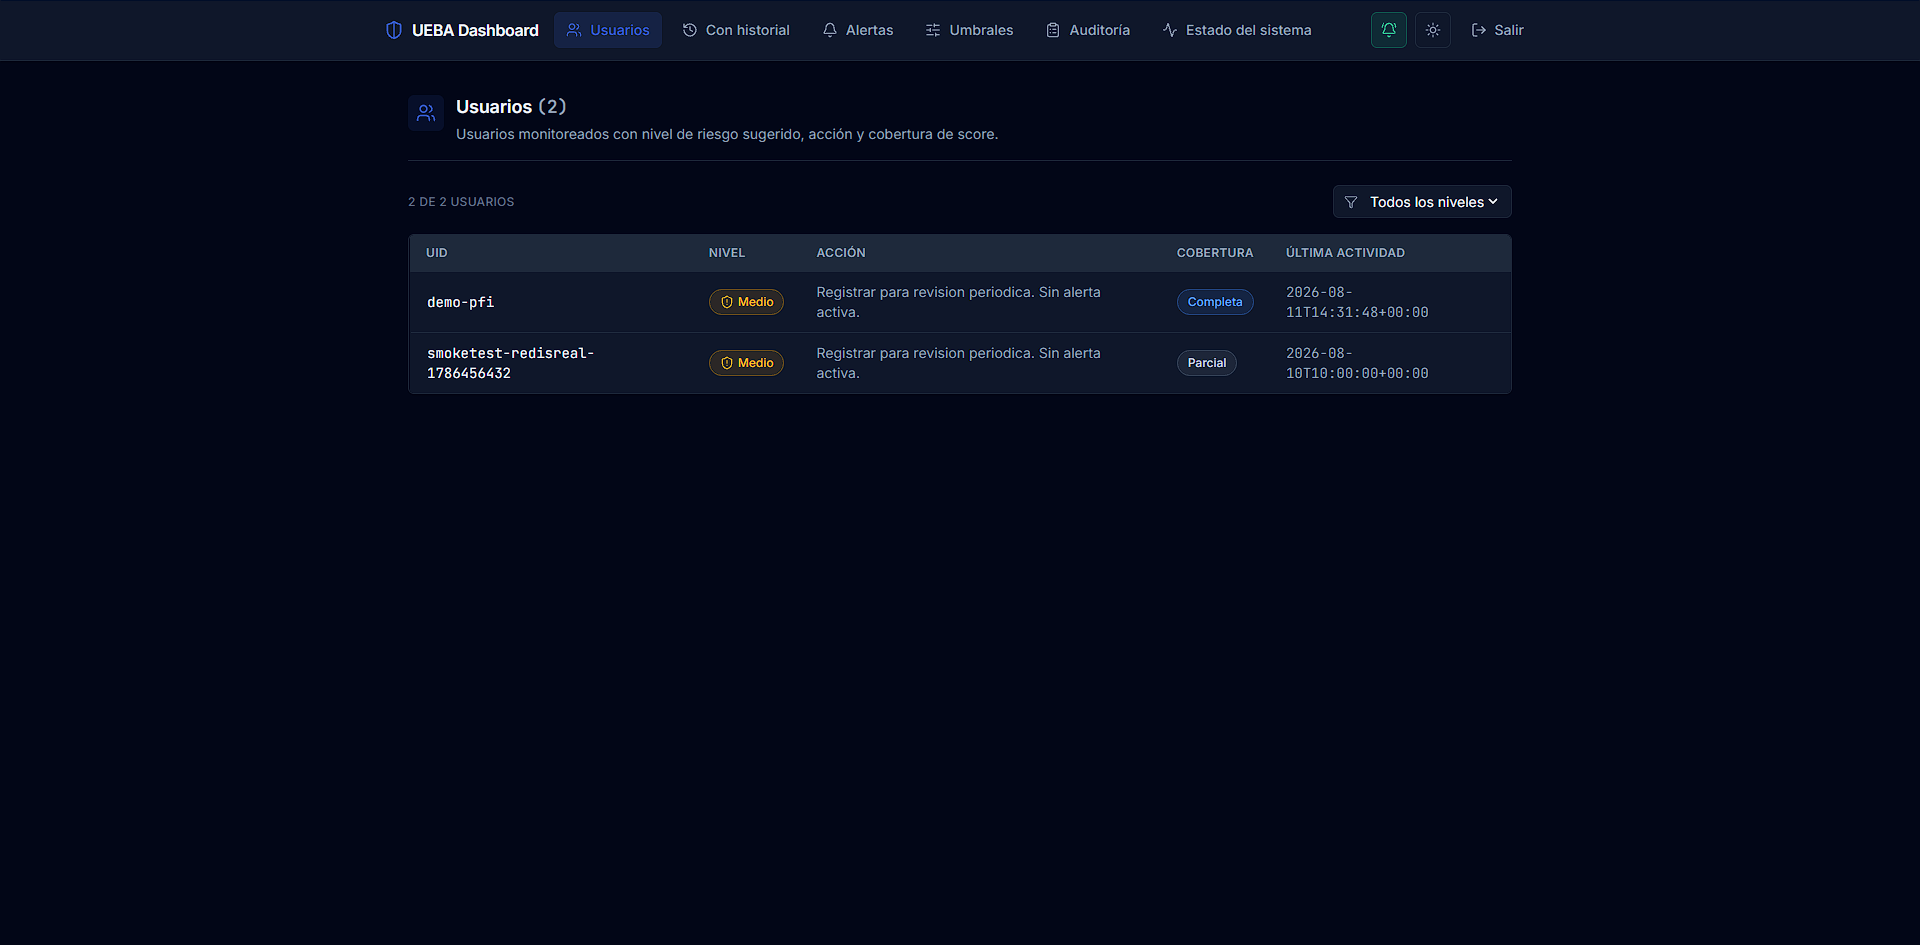
\includegraphics[width=0.8\textwidth]{images/mockups/mockup-usuarios-real.png}
	\caption{Pantalla real: \texttt{/} (listado de usuarios)}
	\label{fig:mockup-usuarios-real}
	{\small Fuente: elaboración propia, captura del sistema.\par}
\end{figure}
\FloatBarrier

\begin{longtable}{p{1.8cm}p{12.8cm}}
	\caption{Justificación de diseño: Usuarios (listado)}
	\label{tab:mockup-usuarios}\\
	\hline
	\textbf{ID} & \textbf{Justificación de diseño} \\
	\hline
	\endfirsthead
	\hline
	\textbf{ID} & \textbf{Justificación de diseño} \\
	\hline
	\endhead
	RF-16 & El listado muestra \emph{score}/nivel de confianza en tiempo real por usuario, con filtro por nivel de riesgo, tal como pide el requerimiento. \\
	\hline
	RNF-15 & El nivel de riesgo se representa con un \emph{badge} de color (bajo/medio/alto/crítico) en lugar de solo un número, permitiendo priorizar de un vistazo (ver Sección~\ref{sec:decisiones-transversales-mockups} para la justificación de la paleta). \\
	\hline
	CU-01 (postcondición) & La acción de mitigación decidida por la API queda visible por usuario, sin que el administrador tenga que consultar \emph{logs} por separado. \\
	\hline
\end{longtable}
\FloatBarrier

\subsection{Detalle de usuario}
Se accede haciendo clic sobre una fila del listado de Usuarios. Profundiza el mismo registro que ya aparece en la tabla (\texttt{uid}, nivel, cobertura) y agrega lo que la vista de lista no puede mostrar sin saturarse: el \emph{score} exacto, la acción sugerida en texto completo, un gráfico de evolución temporal del \emph{score} y el detalle evento por evento que lo originó.

La tarjeta superior repite el mismo par de \emph{badges} (nivel de riesgo y cobertura) que la fila de origen en el listado, para que el administrador reconozca que sigue viendo al mismo usuario y no pierda el contexto al navegar. El \emph{score} se destaca en tipografía grande, por ser el dato que responde más directamente a ``¿qué tan grave es esto ahora?''.

El gráfico de Histórico de \emph{score} aclara explícitamente que el punto ``Actual'' es provisional, porque el día todavía no cerró, y que el resto del histórico solo muestra días ya cerrados. Es la misma decisión de transparencia que ya aparece en Alertas y en Con historial: declarar en la propia pantalla los límites de lo que se está mostrando, en vez de dejar que el administrador asuma que todo el gráfico tiene el mismo nivel de certeza.

La tabla de Eventos recientes está acotada a 20 filas (RF-09) y se aclara que es complementaria al \emph{score} vivo y al histórico diario de arriba, sin reemplazar a ninguno de los dos, evitando que el administrador confunda ``los últimos eventos que vio'' con el historial completo de actividad del usuario. La Figura~\ref{fig:mockup-detalle-wireframe} presenta el \emph{wireframe} de la pantalla y la Figura~\ref{fig:mockup-detalle-real}, la pantalla implementada.

\begin{figure}[t]
	\centering
	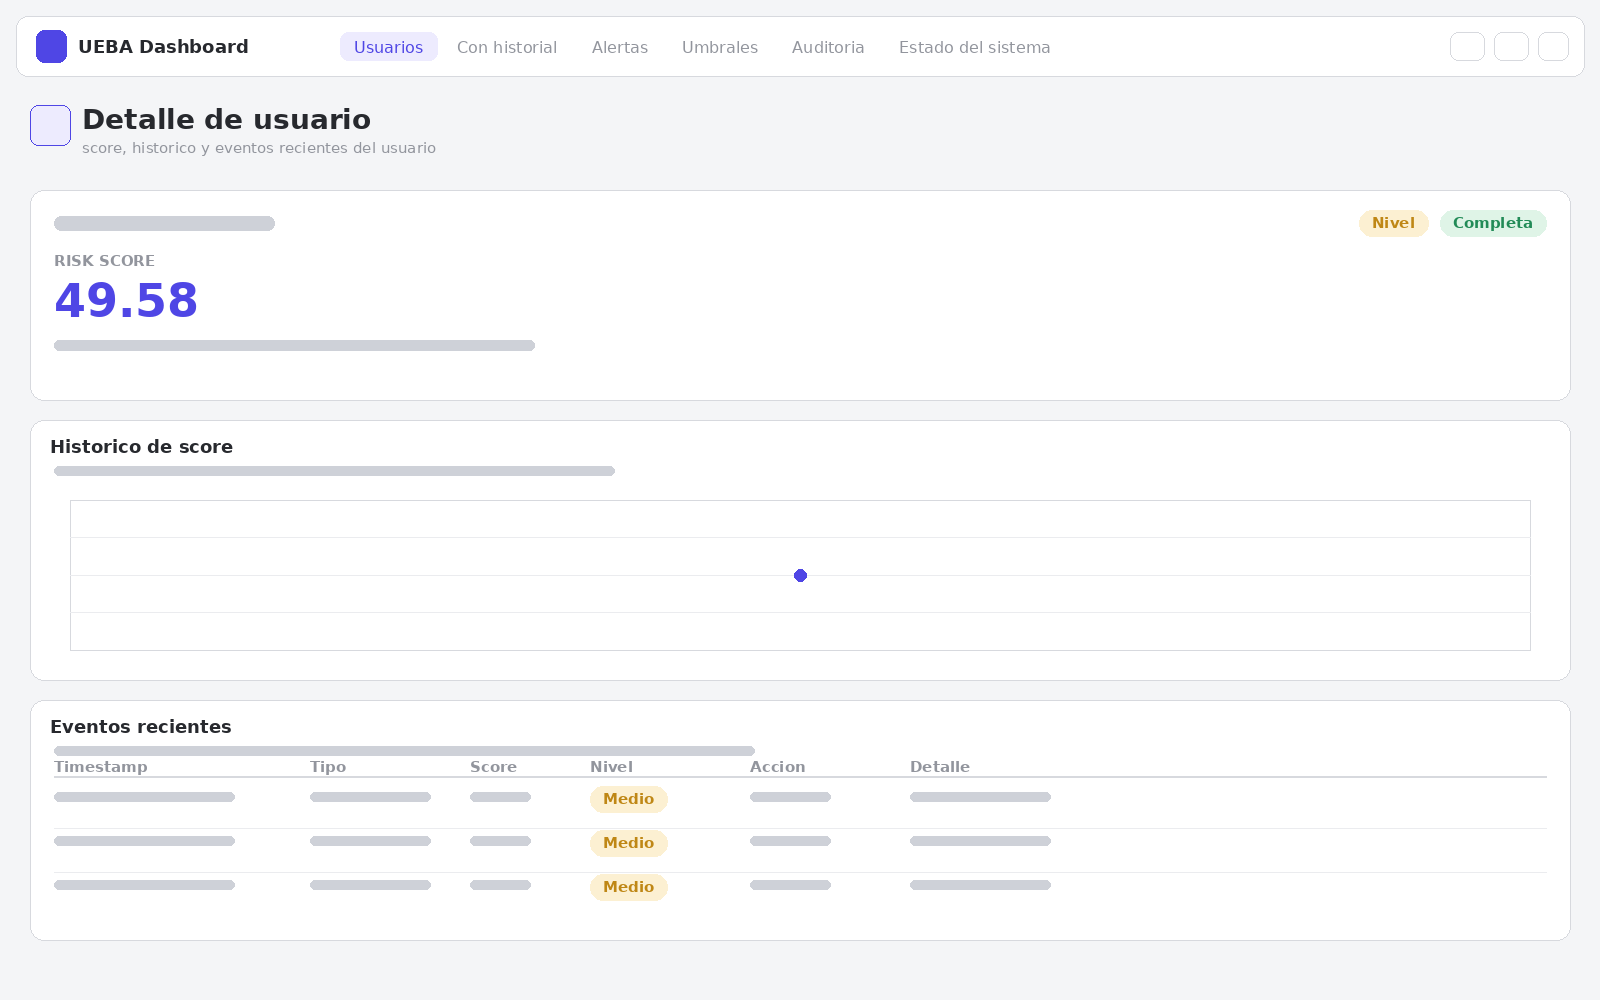
\includegraphics[width=0.8\textwidth]{images/mockups/mockup-detalle-wireframe.png}
	\caption{Wireframe de baja fidelidad: Detalle de usuario}
	\label{fig:mockup-detalle-wireframe}
	{\small Fuente: elaboración propia.\par}
	\bigskip
	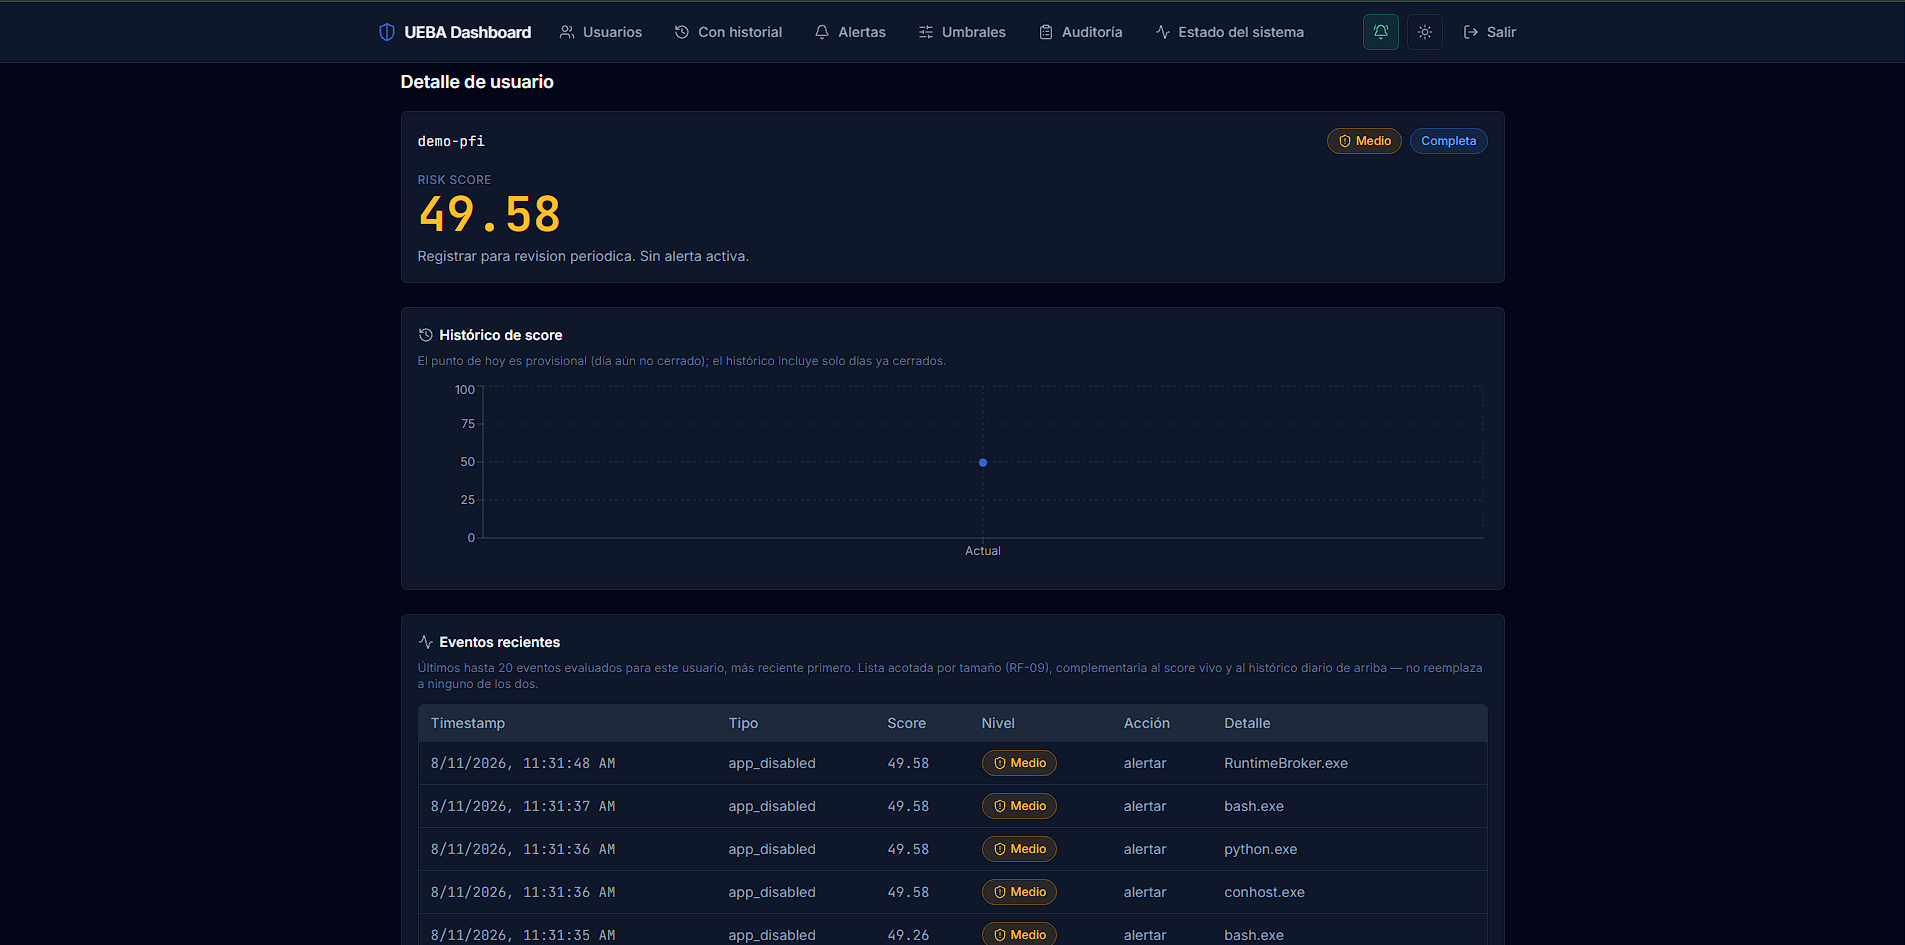
\includegraphics[width=0.8\textwidth]{images/mockups/mockup-detalle-real.png}
	\caption{Pantalla real: \texttt{/usuarios/:uid} (detalle)}
	\label{fig:mockup-detalle-real}
	{\small Fuente: elaboración propia, captura del sistema.\par}
\end{figure}
\FloatBarrier

\begin{longtable}{p{1.8cm}p{12.8cm}}
	\caption{Justificación de diseño: Detalle de usuario}
	\label{tab:mockup-detalle}\\
	\hline
	\textbf{ID} & \textbf{Justificación de diseño} \\
	\hline
	\endfirsthead
	\hline
	\textbf{ID} & \textbf{Justificación de diseño} \\
	\hline
	\endhead
	RF-09 & El límite de 20 eventos evaluados por usuario, con el más reciente primero, está impuesto por requerimiento y comunicado en el propio texto de la sección. \\
	\hline
	RF-16 & Expone el detalle completo de \emph{score} y confianza que el listado general resume en un \emph{badge}, cerrando el flujo ``ver todos'' $\rightarrow$ ``investigar uno''. \\
	\hline
	RNF-15 & Reutiliza los mismos \emph{badges} de nivel de riesgo y el mismo color de acento para el \emph{score} que en Usuarios y Alertas, y lo aplica también al punto del gráfico. \\
	\hline
	RNF-11 (explicabilidad) & El detalle evento por evento (tipo, \emph{score}, nivel, acción, proceso) da trazabilidad de qué generó el \emph{score} actual, no solo el número final. \\
	\hline
\end{longtable}
\FloatBarrier

\subsection{Alertas}
Subconjunto operativo del listado de usuarios: solo los que están en nivel alto o crítico en este momento, pensado para uso durante un incidente activo (no requiere filtrar manualmente el listado completo). El texto bajo el título explicita una limitación de diseño consciente y comunicada al usuario del sistema: no hay historial persistente de alertas ni notificaciones \emph{push}: ``reconocer'' solo oculta el resaltado durante la sesión del navegador. La captura muestra el estado vacío, que es el estado normal del sistema en operación sana. La Figura~\ref{fig:mockup-alertas-wireframe} presenta el \emph{wireframe} de la pantalla y la Figura~\ref{fig:mockup-alertas-real}, la pantalla implementada.

\begin{figure}[t]
	\centering
	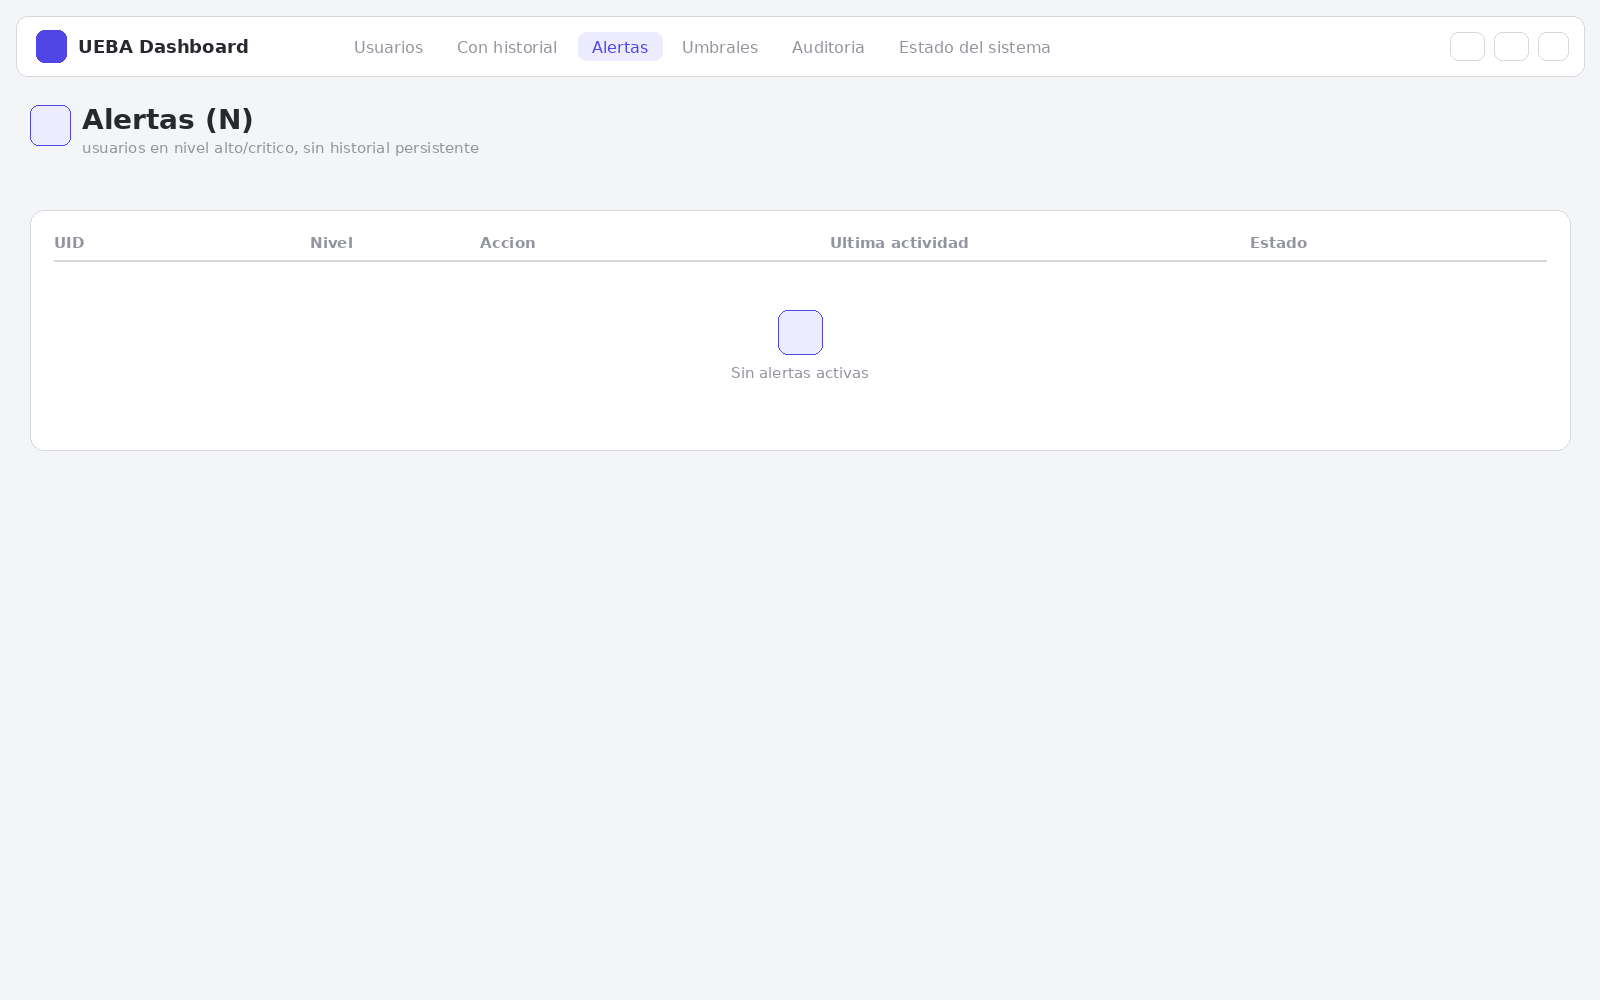
\includegraphics[width=0.8\textwidth]{images/mockups/mockup-alertas-wireframe.png}
	\caption{Wireframe de baja fidelidad: Alertas}
	\label{fig:mockup-alertas-wireframe}
	{\small Fuente: elaboración propia.\par}
	\bigskip
	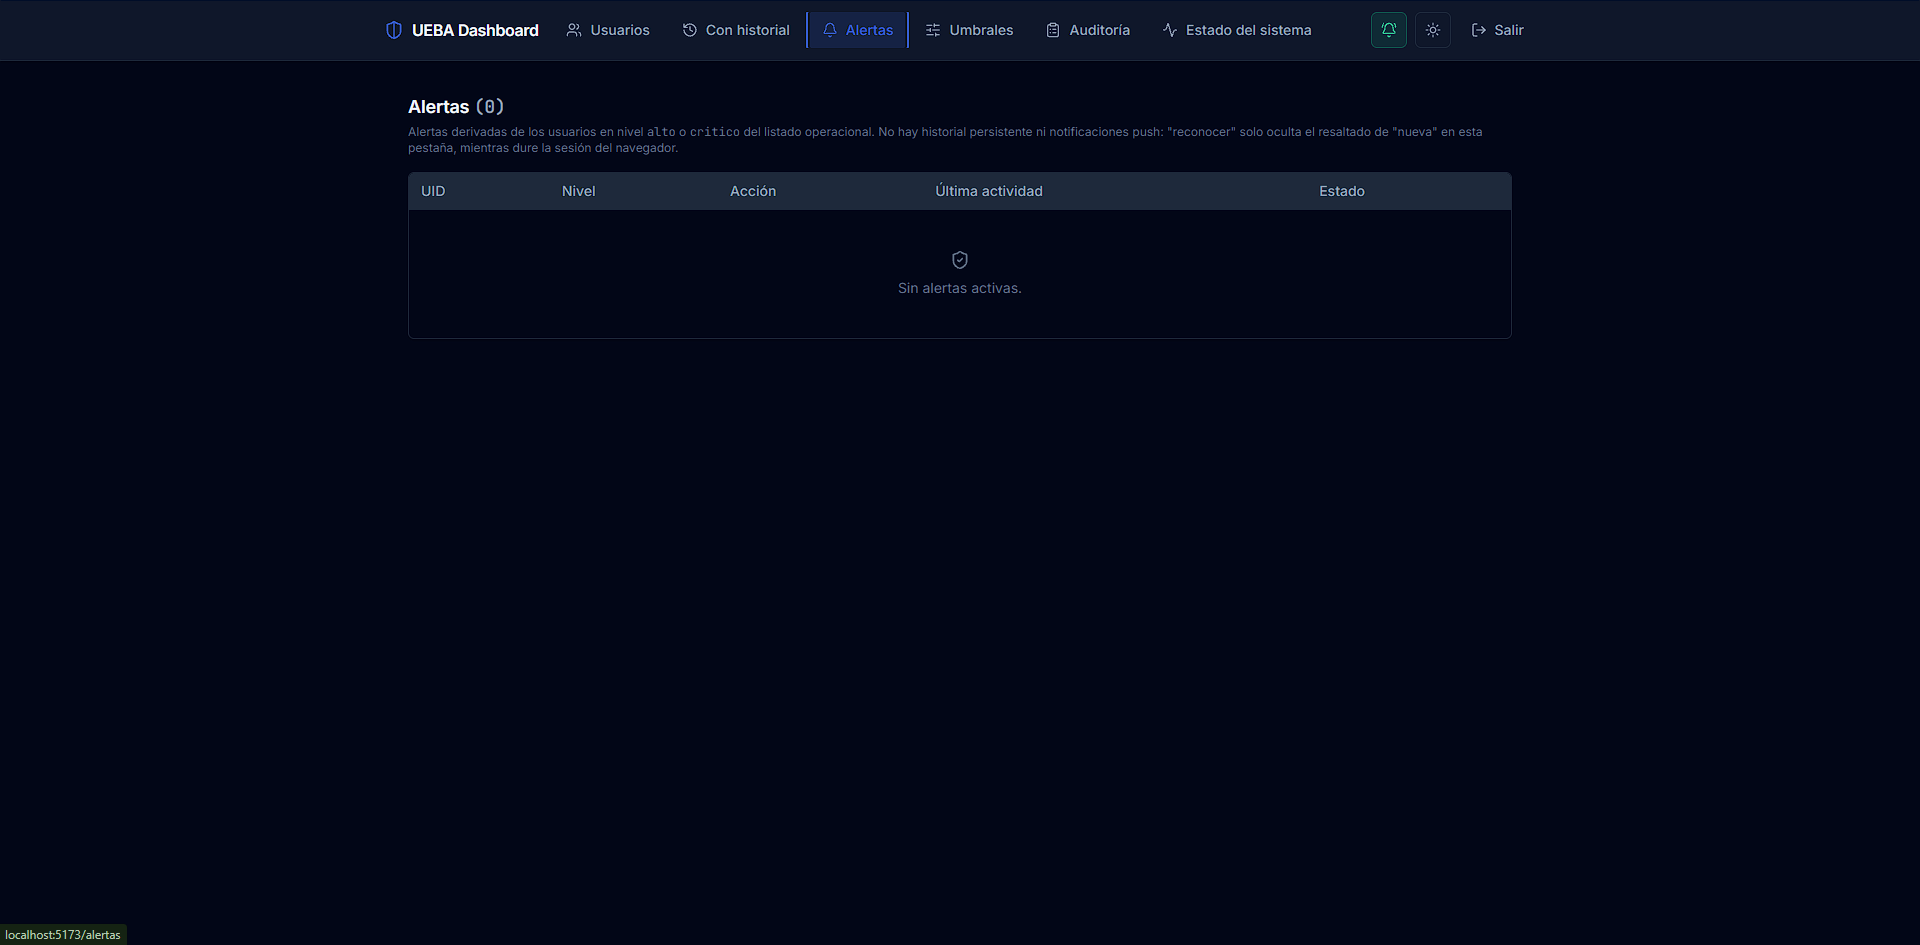
\includegraphics[width=0.8\textwidth]{images/mockups/mockup-alertas-real.png}
	\caption{Pantalla real: \texttt{/alertas} (estado vacío)}
	\label{fig:mockup-alertas-real}
	{\small Fuente: elaboración propia, captura del sistema.\par}
\end{figure}
\FloatBarrier

\begin{longtable}{p{1.8cm}p{12.8cm}}
	\caption{Justificación de diseño: Alertas}
	\label{tab:mockup-alertas}\\
	\hline
	\textbf{ID} & \textbf{Justificación de diseño} \\
	\hline
	\endfirsthead
	\hline
	\textbf{ID} & \textbf{Justificación de diseño} \\
	\hline
	\endhead
	RNF-15 & Reutiliza el mismo patrón visual de \emph{badges} de nivel que el listado general, manteniendo consistencia y evitando que el administrador tenga que reaprender la codificación de color. \\
	\hline
	Transparencia de diseño & El límite del mecanismo (sin persistencia, sin \emph{push}) se declara en la propia pantalla en vez de dar a entender una capacidad de alertado que el sistema no tiene: es una decisión deliberada para no sobre-prometer funcionalidad. \\
	\hline
\end{longtable}
\FloatBarrier

\subsection{Configuración de umbrales}
Es la pantalla de mayor densidad funcional del \emph{dashboard}: concentra los 4 sub-formularios que dan cumplimiento a CU-02 completo (RF-12 a RF-15 y RF-17; la periodicidad corresponde a RF-18). Se organiza en secciones apiladas con jerarquía clara (Umbrales por nivel arriba, luego una grilla de dos columnas con Acción por nivel y Periodicidad de reentrenamiento, y Notificaciones al final), cada una con su propio botón de guardado independiente, lo que evita que un cambio de umbral dispare accidentalmente un guardado de notificaciones.

El bloque de Notificaciones usa \emph{chips} tipo \emph{toggle} (uno por nivel de riesgo) en vez de \emph{checkboxes} sueltos: permite seleccionar varios niveles a la vez con el mismo patrón visual que los \emph{badges} de riesgo del resto del sistema, en lugar de un control de formulario genérico sin relación visual con el dominio. La Figura~\ref{fig:mockup-umbrales-wireframe} presenta el \emph{wireframe} de la pantalla y las Figuras~\ref{fig:mockup-umbrales-real-1} y~\ref{fig:mockup-umbrales-real-2}, la pantalla implementada en su parte superior y luego de desplazarse.

\begin{figure}[t]
	\centering
	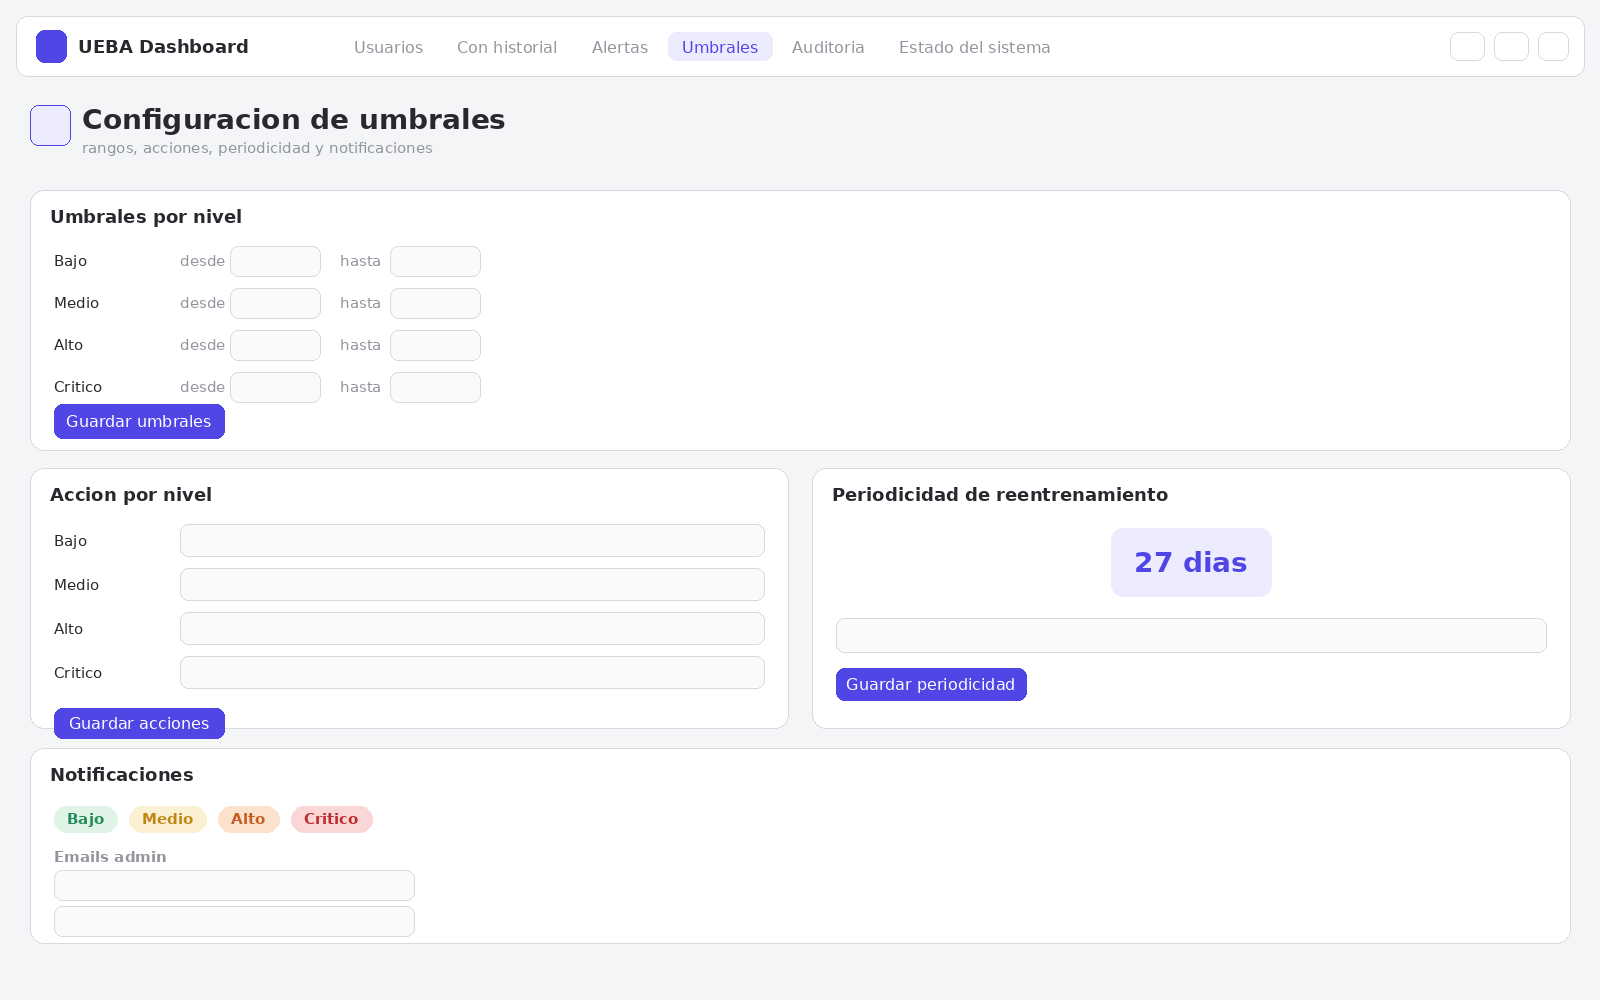
\includegraphics[width=0.68\textwidth]{images/mockups/mockup-umbrales-wireframe.png}
	\caption{Wireframe de baja fidelidad: Configuración de umbrales}
	\label{fig:mockup-umbrales-wireframe}
	{\small Fuente: elaboración propia.\par}
	\bigskip
	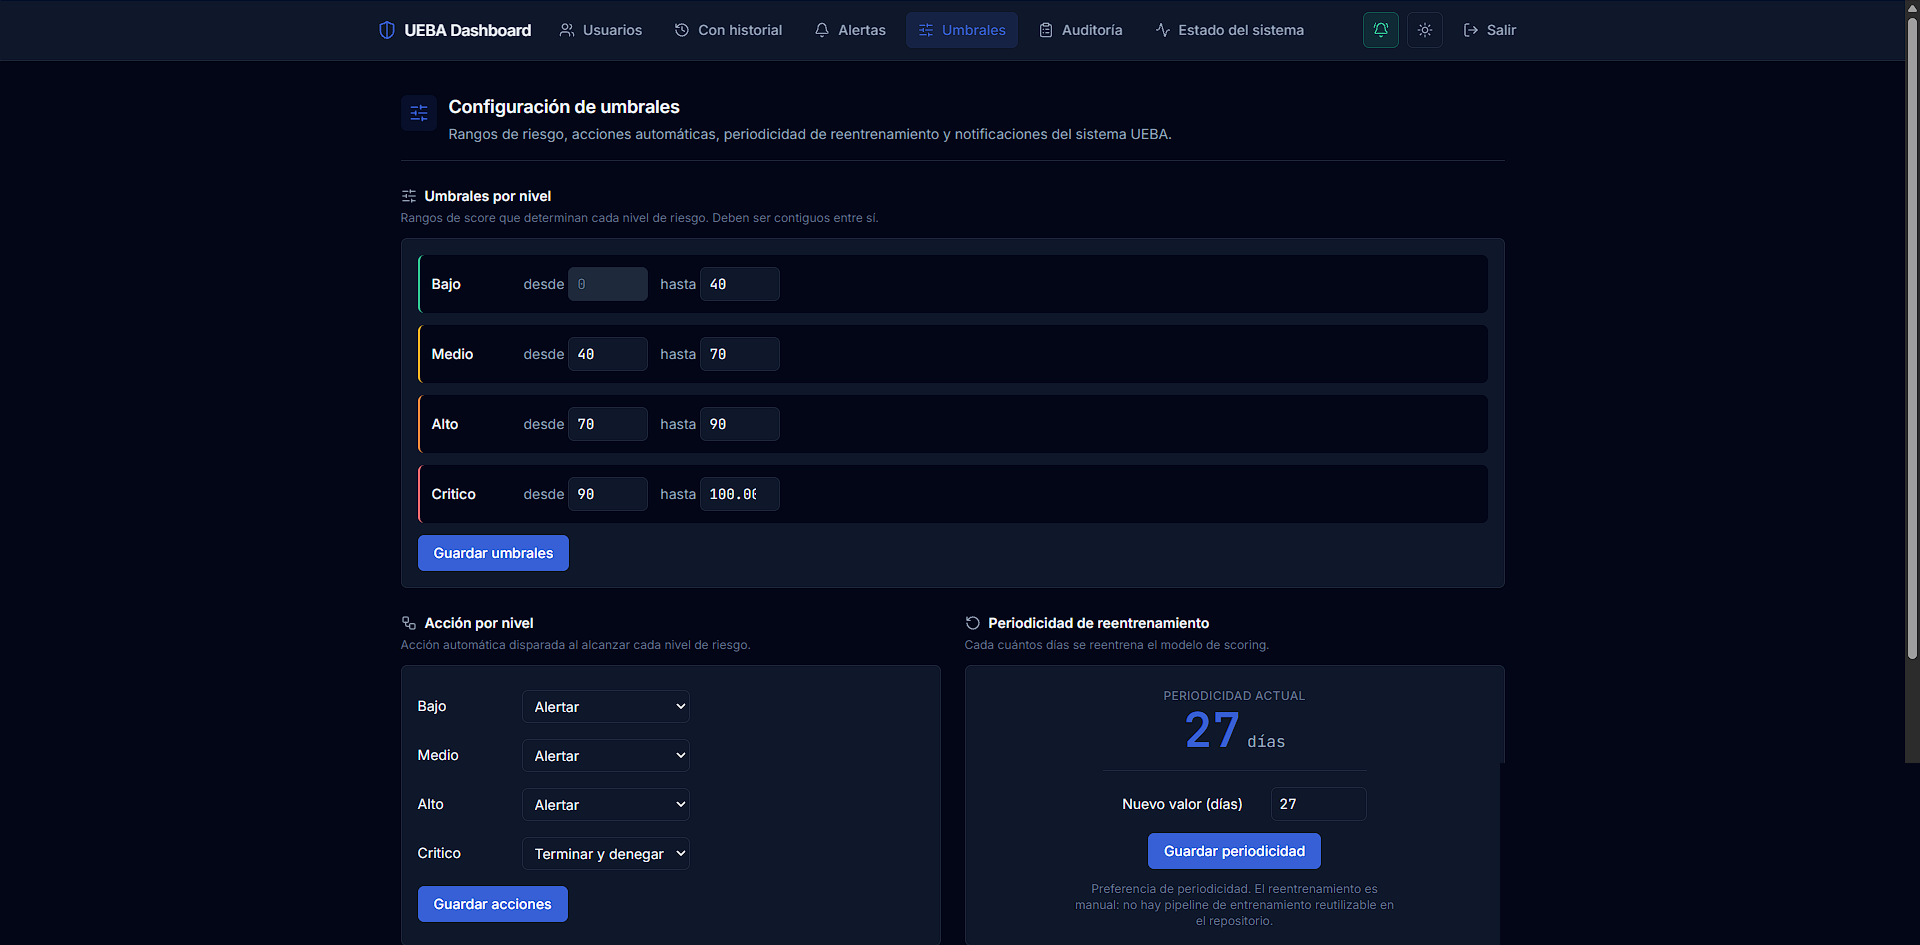
\includegraphics[width=0.68\textwidth]{images/mockups/mockup-umbrales-real-1.png}
	\caption{Pantalla real: \texttt{/umbrales} (parte superior: rangos por nivel)}
	\label{fig:mockup-umbrales-real-1}
	{\small Fuente: elaboración propia, captura del sistema.\par}
	\bigskip
	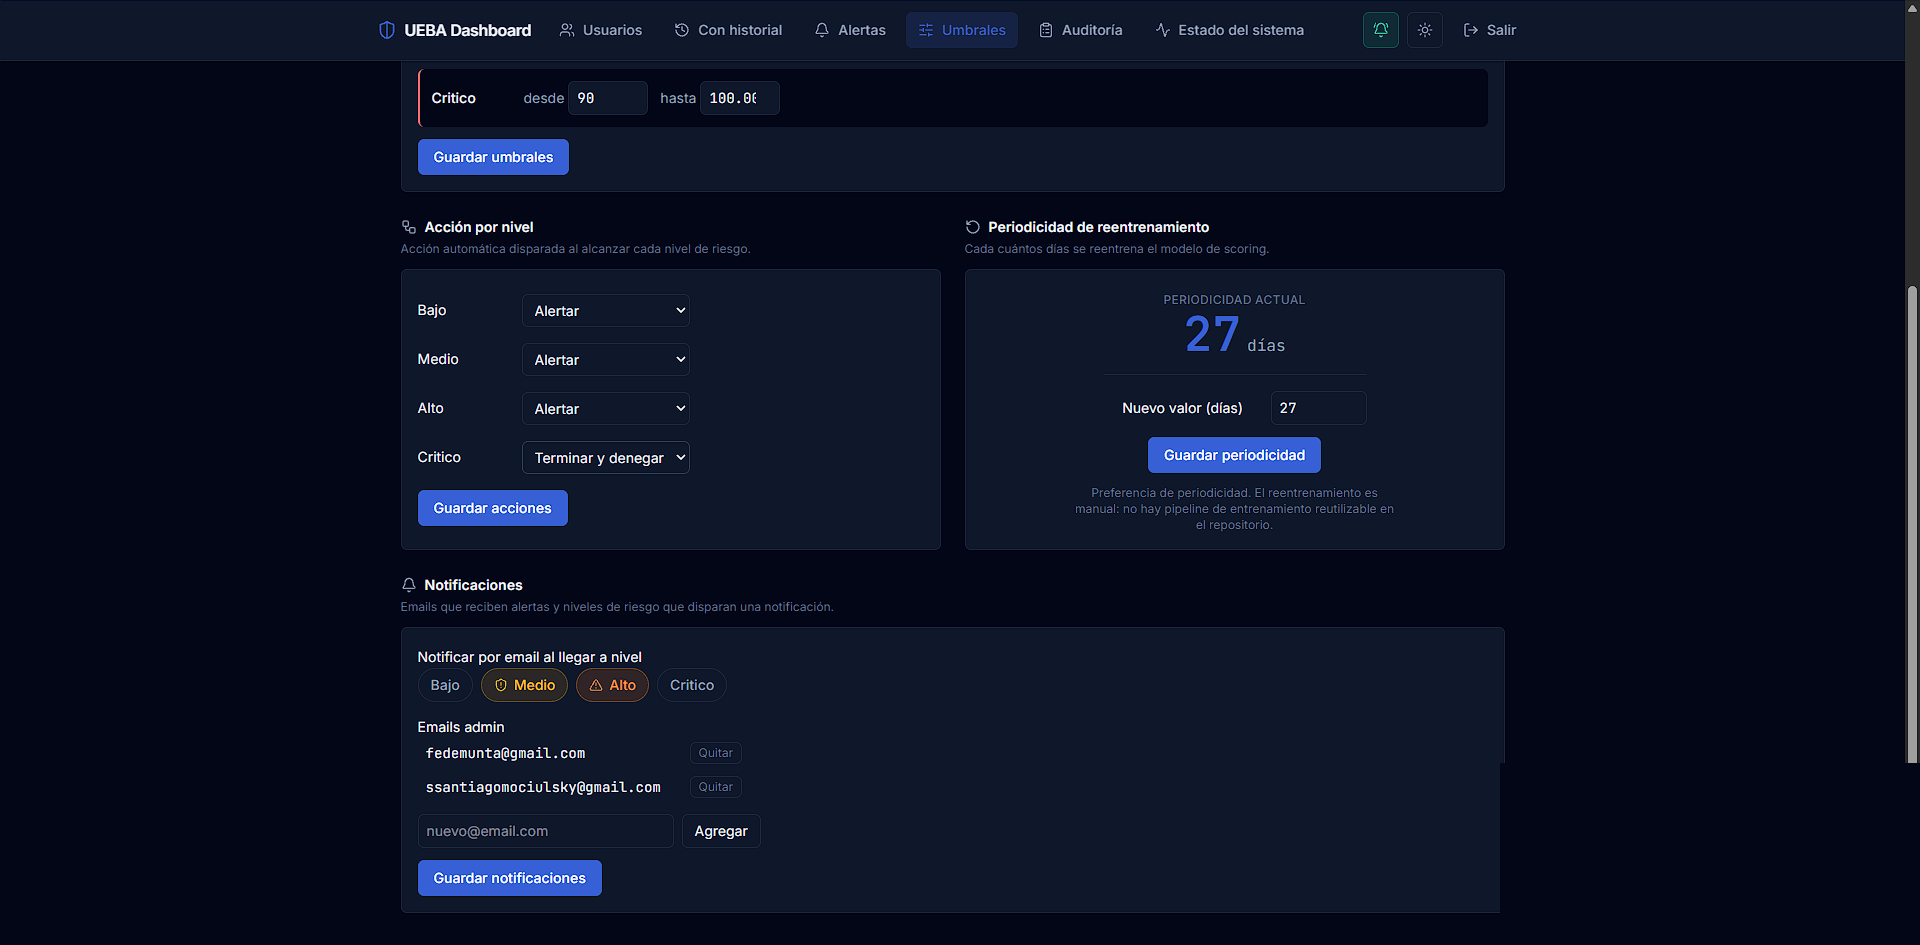
\includegraphics[width=0.68\textwidth]{images/mockups/mockup-umbrales-real-2.png}
	\caption{Pantalla real: \texttt{/umbrales} (scroll: acciones, periodicidad y notificaciones)}
	\label{fig:mockup-umbrales-real-2}
	{\small Fuente: elaboración propia, captura del sistema.\par}
\end{figure}
\FloatBarrier

\begin{longtable}{p{1.8cm}p{12.8cm}}
	\caption{Justificación de diseño: Configuración de umbrales}
	\label{tab:mockup-umbrales}\\
	\hline
	\textbf{ID} & \textbf{Justificación de diseño} \\
	\hline
	\endfirsthead
	\hline
	\textbf{ID} & \textbf{Justificación de diseño} \\
	\hline
	\endhead
	RF-12, RF-14, RF-15, RF-18 & Cada sub-formulario (umbrales, acciones, periodicidad, notificaciones) envía su propio \texttt{PUT} independiente al \emph{endpoint} de configuración correspondiente, reflejado en la separación visual de secciones con su propio botón. \\
	\hline
	RF-12 & Los campos de umbral están dispuestos en pares desde/hasta contiguos por nivel, facilitando detectar visualmente un solapamiento antes de guardar (aunque la validación real ocurre del lado de la API). \\
	\hline
	RNF-07 & Todo el formulario opera en caliente contra la API, sin ningún paso de reinicio: el diseño no incluye ninguna acción de tipo ``aplicar y reiniciar''. \\
	\hline
	RNF-15 / consistencia & Los \emph{chips} de Notificaciones reutilizan la misma forma visual (\emph{badge} redondeado, color por nivel) que el resto de las pantallas usa para representar niveles de riesgo. \\
	\hline
\end{longtable}
\FloatBarrier

\subsection{Auditoría}
Traduce directamente a RF-17 (historial de versiones de política, visible desde el \emph{dashboard}, para trazabilidad). Cada entrada es una tarjeta con el tipo de cambio (Acción por nivel, Periodicidad, Notificaciones), el valor anterior y el nuevo en formato monoespaciado tipo \emph{diff}, más fecha/hora y actor. El formato \emph{diff} (\texttt{valor\_viejo} $\rightarrow$ \texttt{valor\_nuevo}) se elige en vez de mostrar solo el estado final, porque el propósito de esta pantalla es auditar cambios, no solo consultar configuración actual: para eso ya está \texttt{/umbrales}. La Figura~\ref{fig:mockup-auditoria-wireframe} presenta el \emph{wireframe} de la pantalla y la Figura~\ref{fig:mockup-auditoria-real}, la pantalla implementada.

\begin{figure}[t]
	\centering
	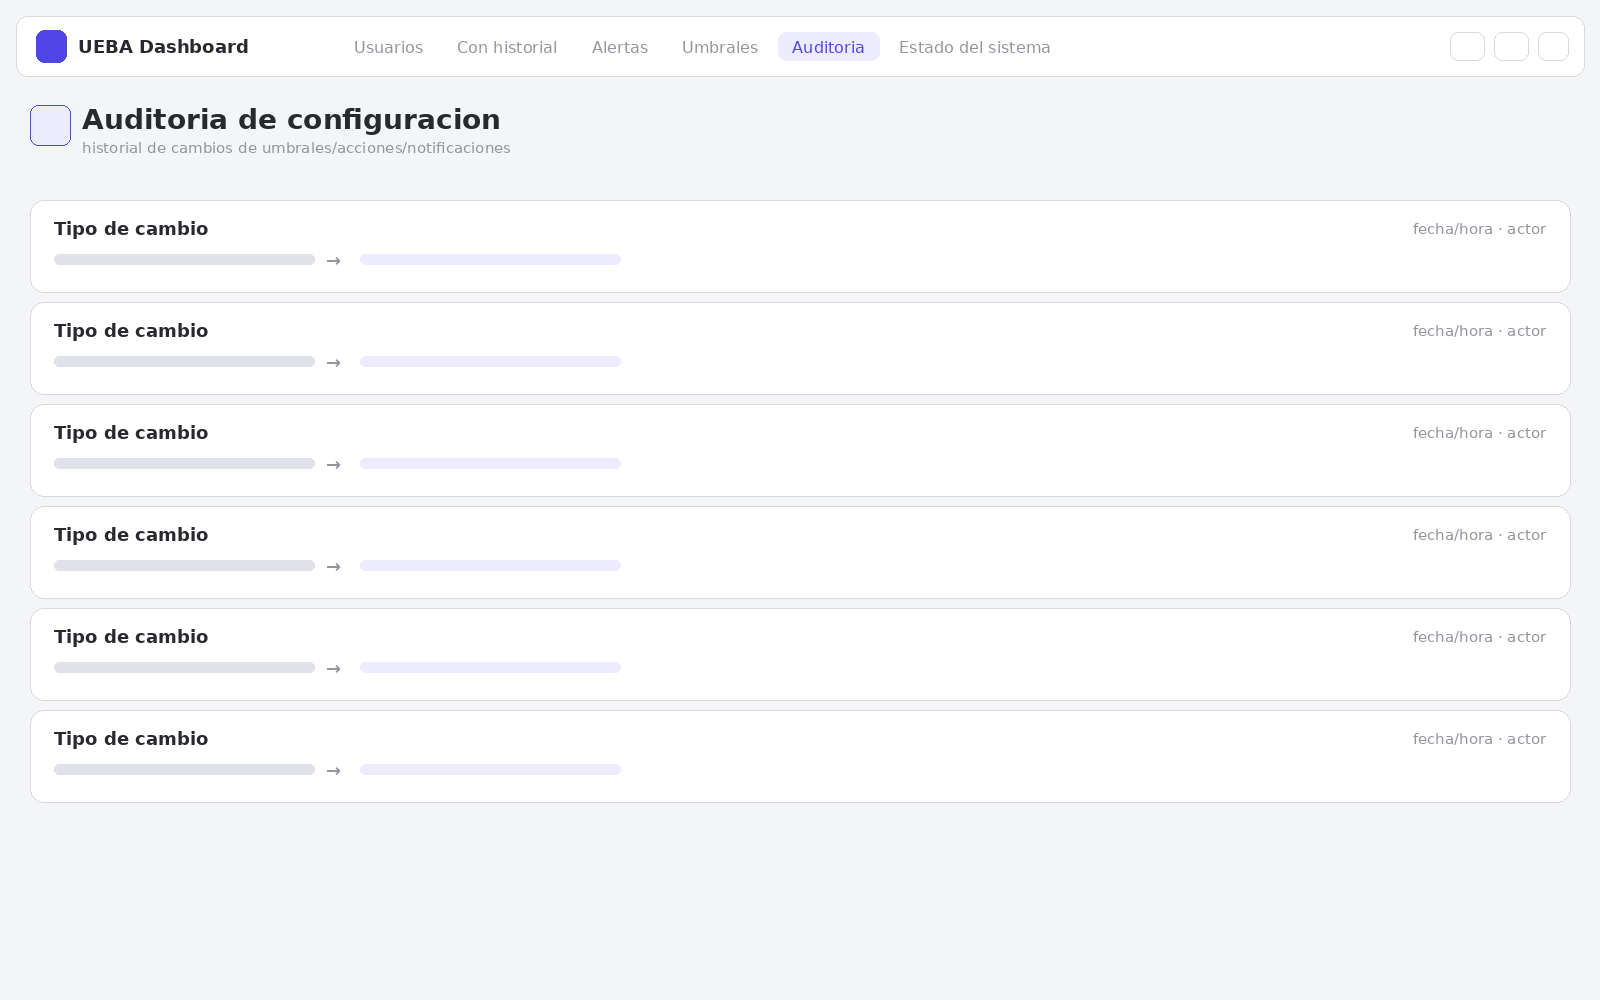
\includegraphics[width=0.8\textwidth]{images/mockups/mockup-auditoria-wireframe.png}
	\caption{Wireframe de baja fidelidad: Auditoría}
	\label{fig:mockup-auditoria-wireframe}
	{\small Fuente: elaboración propia.\par}
	\bigskip
	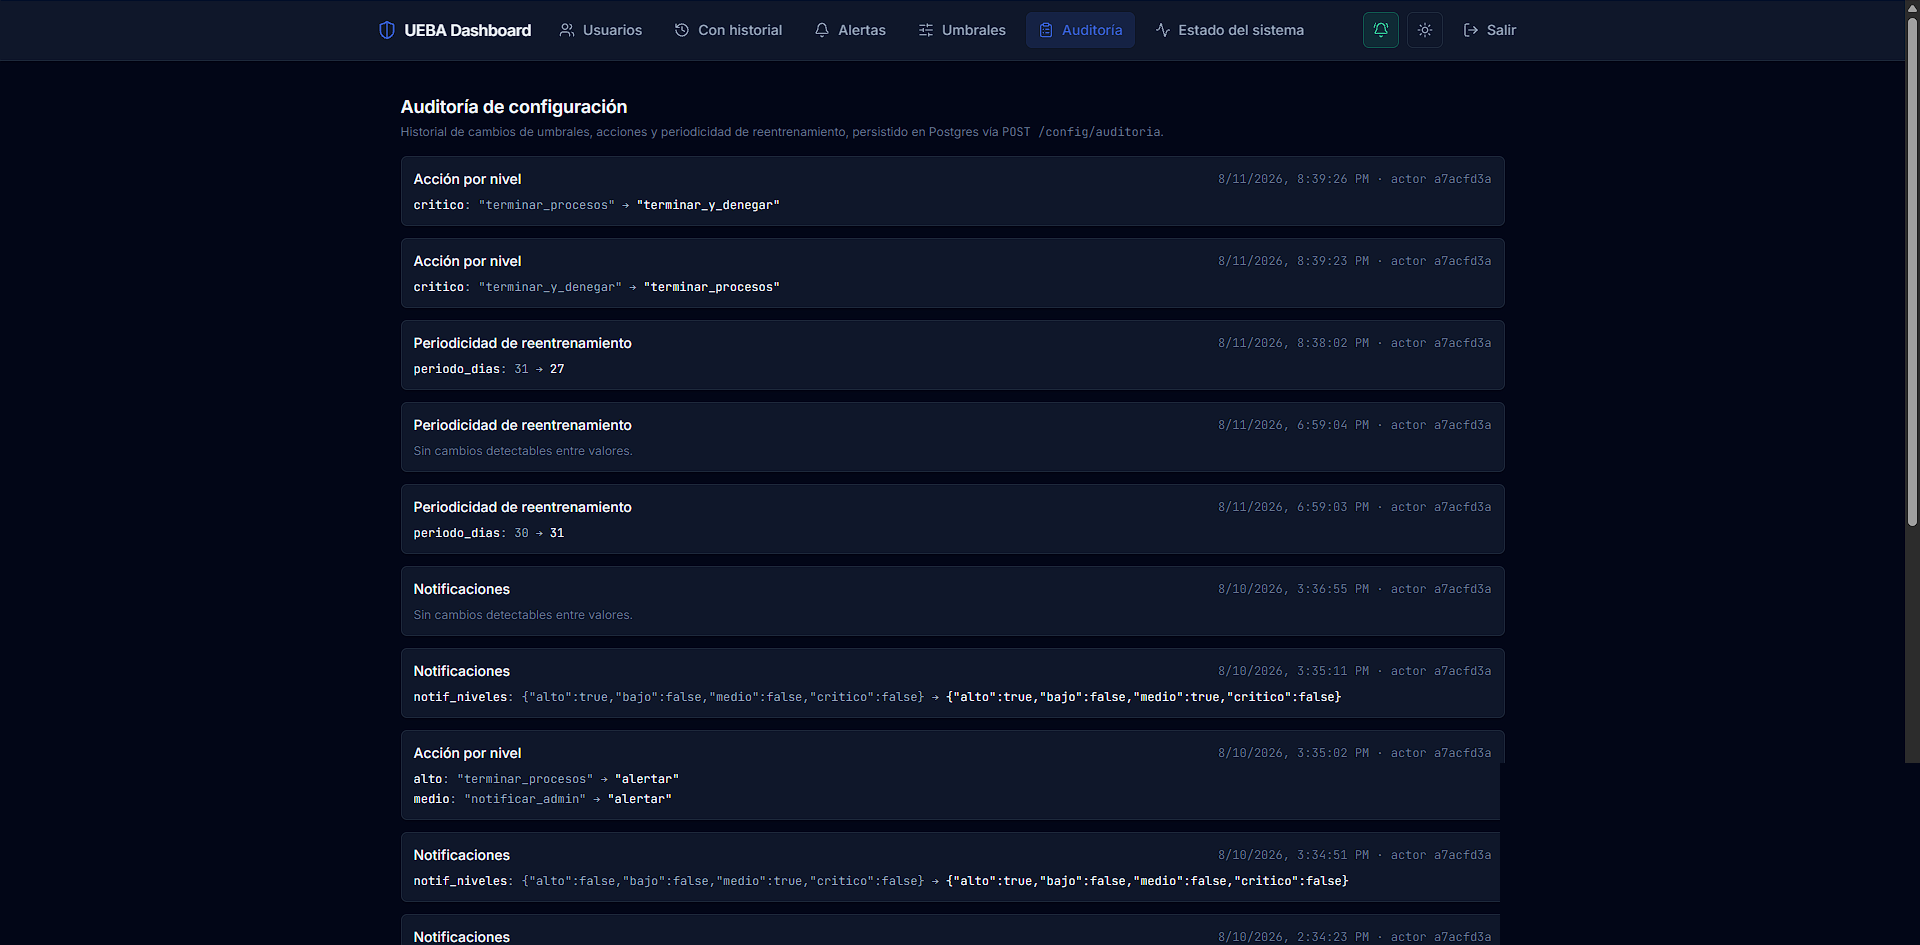
\includegraphics[width=0.8\textwidth]{images/mockups/mockup-auditoria-real.png}
	\caption{Pantalla real: \texttt{/auditoria}}
	\label{fig:mockup-auditoria-real}
	{\small Fuente: elaboración propia, captura del sistema.\par}
\end{figure}
\FloatBarrier

\begin{longtable}{p{1.8cm}p{12.8cm}}
	\caption{Justificación de diseño: Auditoría}
	\label{tab:mockup-auditoria}\\
	\hline
	\textbf{ID} & \textbf{Justificación de diseño} \\
	\hline
	\endfirsthead
	\hline
	\textbf{ID} & \textbf{Justificación de diseño} \\
	\hline
	\endhead
	RF-17 & Historial de versiones de políticas visible desde el \emph{dashboard}, orden cronológico descendente, con actor de cada cambio. \\
	\hline
	RNF-11 (explicabilidad, parcial) & Mostrar el delta exacto (campo, valor anterior, valor nuevo) en lugar de solo un mensaje genérico de ``configuración actualizada'' da trazabilidad concreta de qué cambió y quién lo cambió. \\
	\hline
\end{longtable}
\FloatBarrier

\subsection{Estado del sistema}
Pantalla de verificación técnica: expone el resultado de \texttt{/health} de la API (estado agregado, artefactos del modelo cargados, conectividad a Redis y Postgres) y el detalle de cada artefacto individual (\texttt{isolation\_forest}, \texttt{lstm\_autoencoder}, \emph{scalers}, \emph{encoding}, umbrales del modelo, referencias de entrenamiento). No es una pantalla pensada para uso operativo diario del administrador de seguridad, sino como herramienta de verificación rápida de que el sistema está sano. Por eso se incluye en este relevamiento pese a no derivar de un requerimiento funcional puntual: documenta una decisión de diseño real (visibilidad de salud técnica del sistema) aunque su alcance sea acotado y esté sujeta a revisión. La Figura~\ref{fig:mockup-estado-wireframe} presenta el \emph{wireframe} de la pantalla y la Figura~\ref{fig:mockup-estado-real}, la pantalla implementada.

\begin{figure}[t]
	\centering
	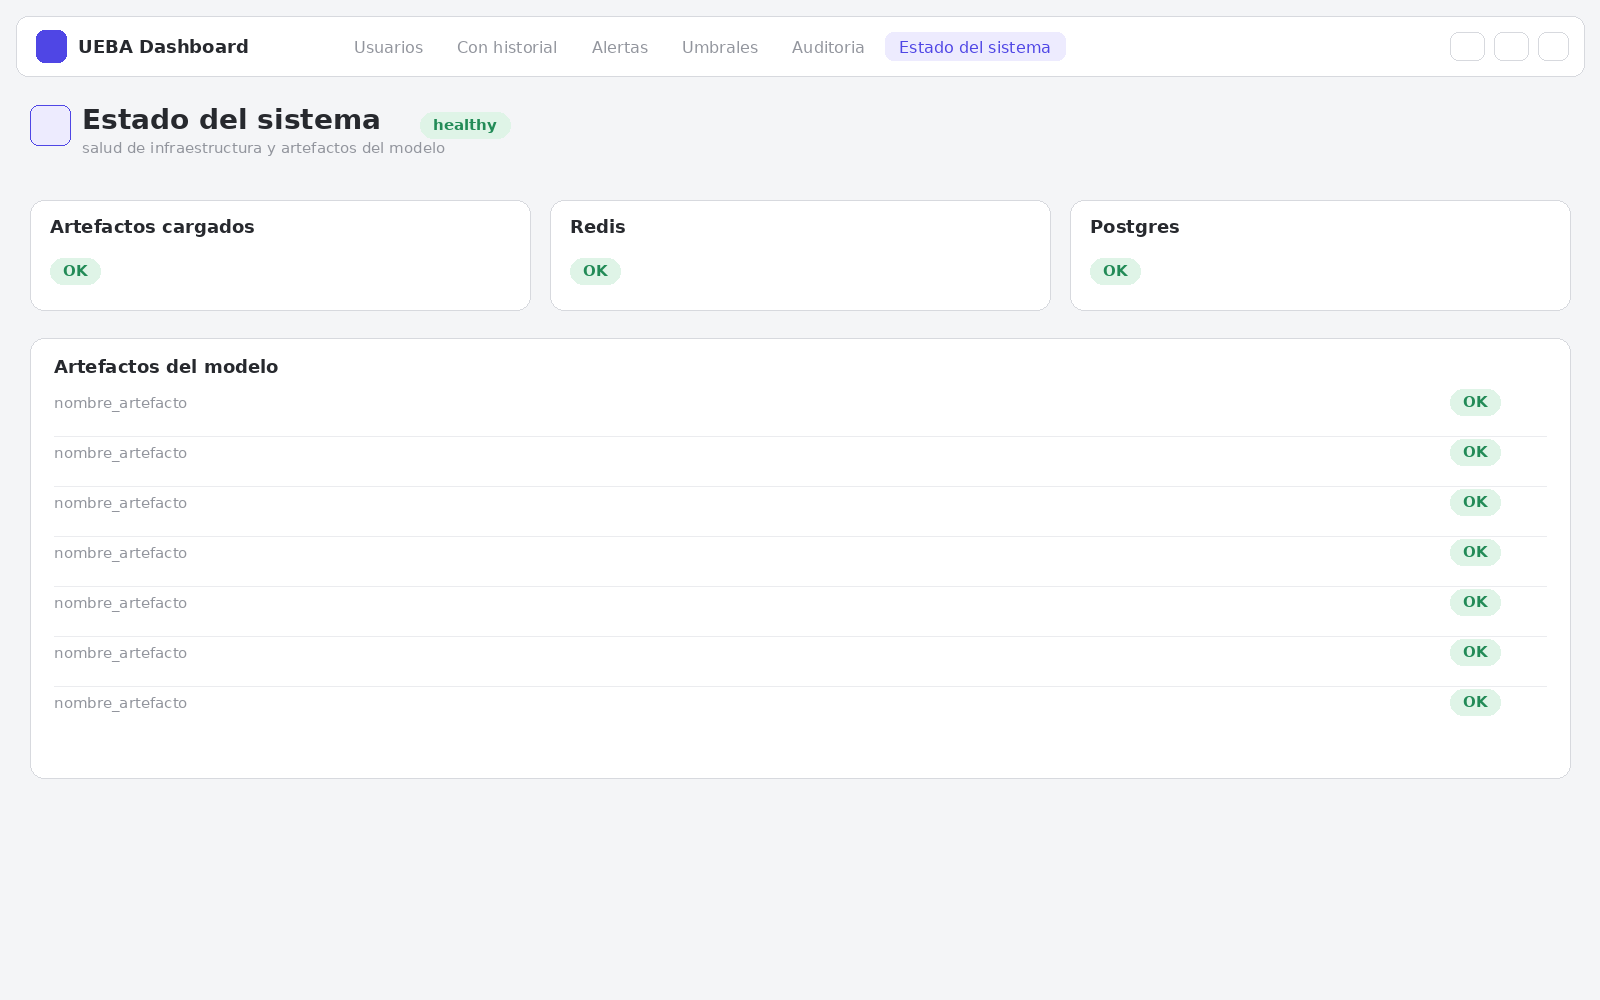
\includegraphics[width=0.8\textwidth]{images/mockups/mockup-estado-wireframe.png}
	\caption{Wireframe de baja fidelidad: Estado del sistema}
	\label{fig:mockup-estado-wireframe}
	{\small Fuente: elaboración propia.\par}
	\bigskip
	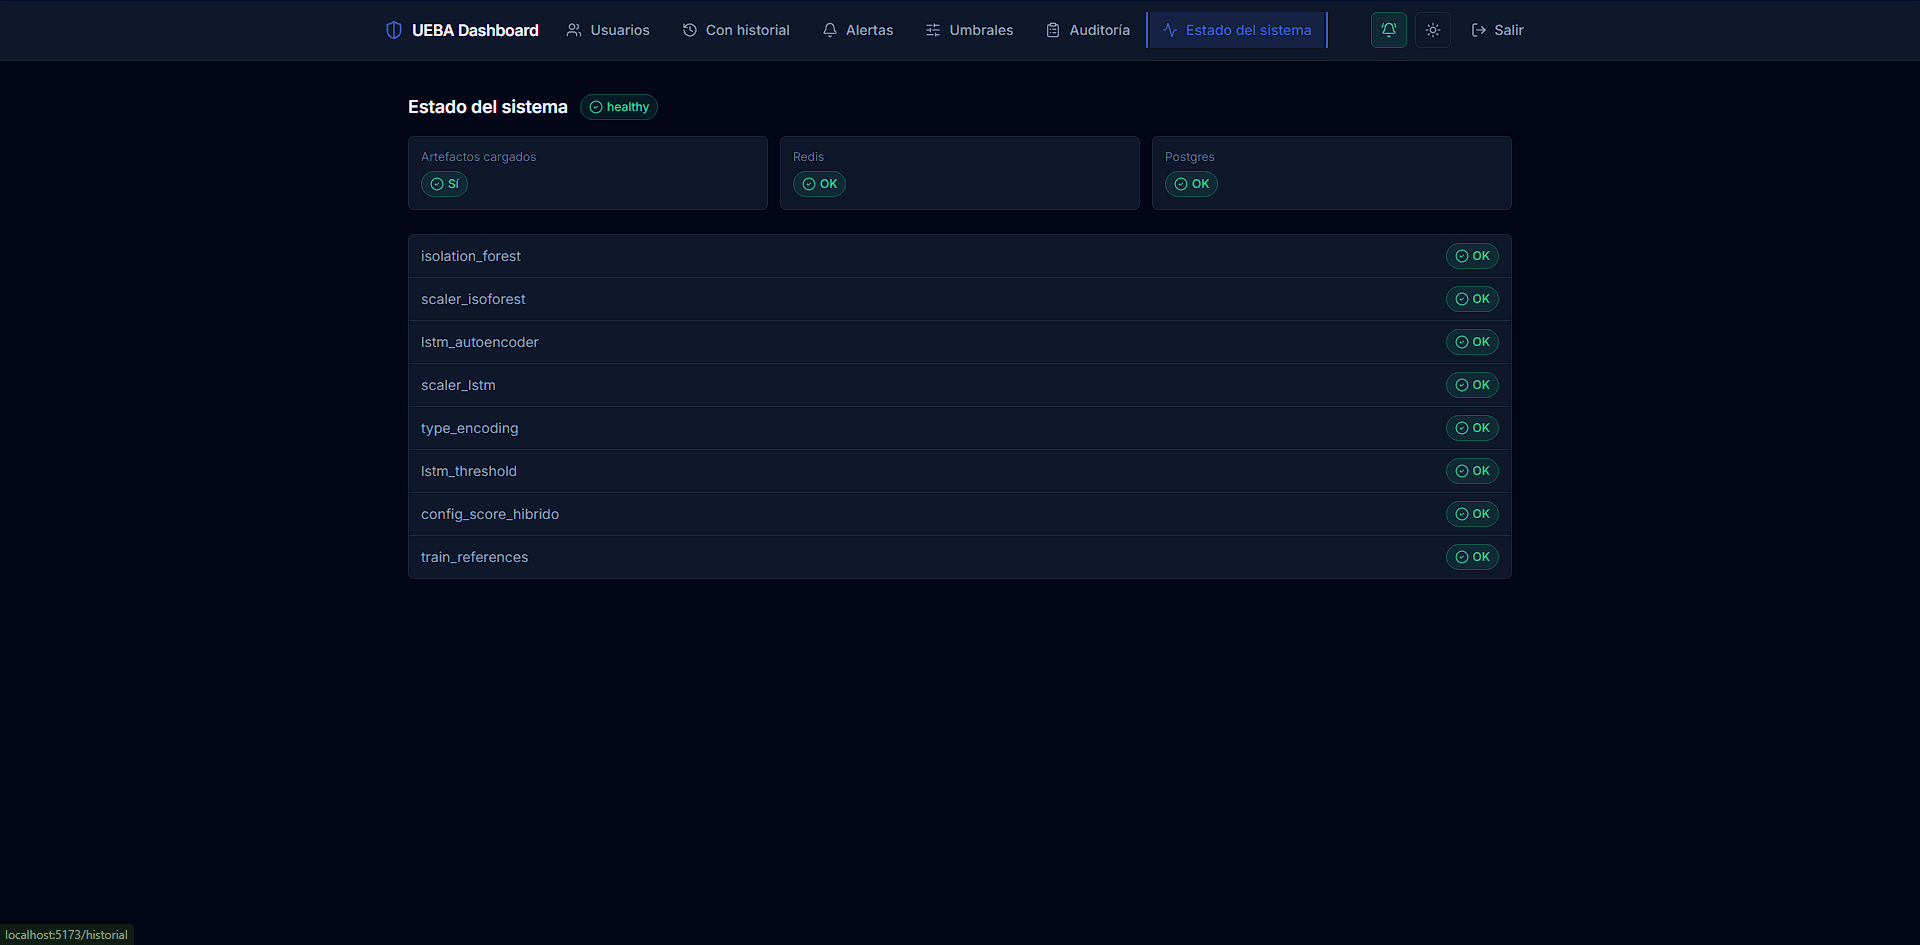
\includegraphics[width=0.8\textwidth]{images/mockups/mockup-estado-real.png}
	\caption{Pantalla real: \texttt{/salud}}
	\label{fig:mockup-estado-real}
	{\small Fuente: elaboración propia, captura del sistema.\par}
\end{figure}
\FloatBarrier

\begin{longtable}{p{1.8cm}p{12.8cm}}
	\caption{Justificación de diseño: Estado del sistema}
	\label{tab:mockup-estado}\\
	\hline
	\textbf{ID} & \textbf{Justificación de diseño} \\
	\hline
	\endfirsthead
	\hline
	\textbf{ID} & \textbf{Justificación de diseño} \\
	\hline
	\endhead
	RNF-15 (aplicado a estado técnico) & Mismo lenguaje visual de \emph{badges} de estado (OK / \emph{healthy}) que el resto del sistema usa para nivel de riesgo, aplicado aquí a salud de infraestructura en vez de riesgo de usuario. \\
	\hline
\end{longtable}
\FloatBarrier

\subsection{Con historial}
Filtra el listado de usuarios a los que ya tienen al menos un día cerrado en \texttt{historial\_scores} (Postgres), como acceso rápido a usuarios con evolución temporal registrada. Es una vista deliberadamente angosta (una sola columna, UID) frente al listado general de Usuarios: no repite \emph{score}/nivel/acción porque esos datos ya cambiaron desde que se cerró ese día: mostrarlos aquí induciría a leerlos como estado actual cuando son historial. El texto bajo el título aclara explícitamente que esta lista (Postgres) puede diferir del listado operacional (Redis): un \texttt{uid} reseteado en Redis conserva igual su historial aquí, y esa distinción se declara en la propia pantalla en lugar de dejarla implícita. La Figura~\ref{fig:mockup-historial-wireframe} presenta el \emph{wireframe} de la pantalla y la Figura~\ref{fig:mockup-historial-real}, la pantalla implementada.

\begin{figure}[t]
	\centering
	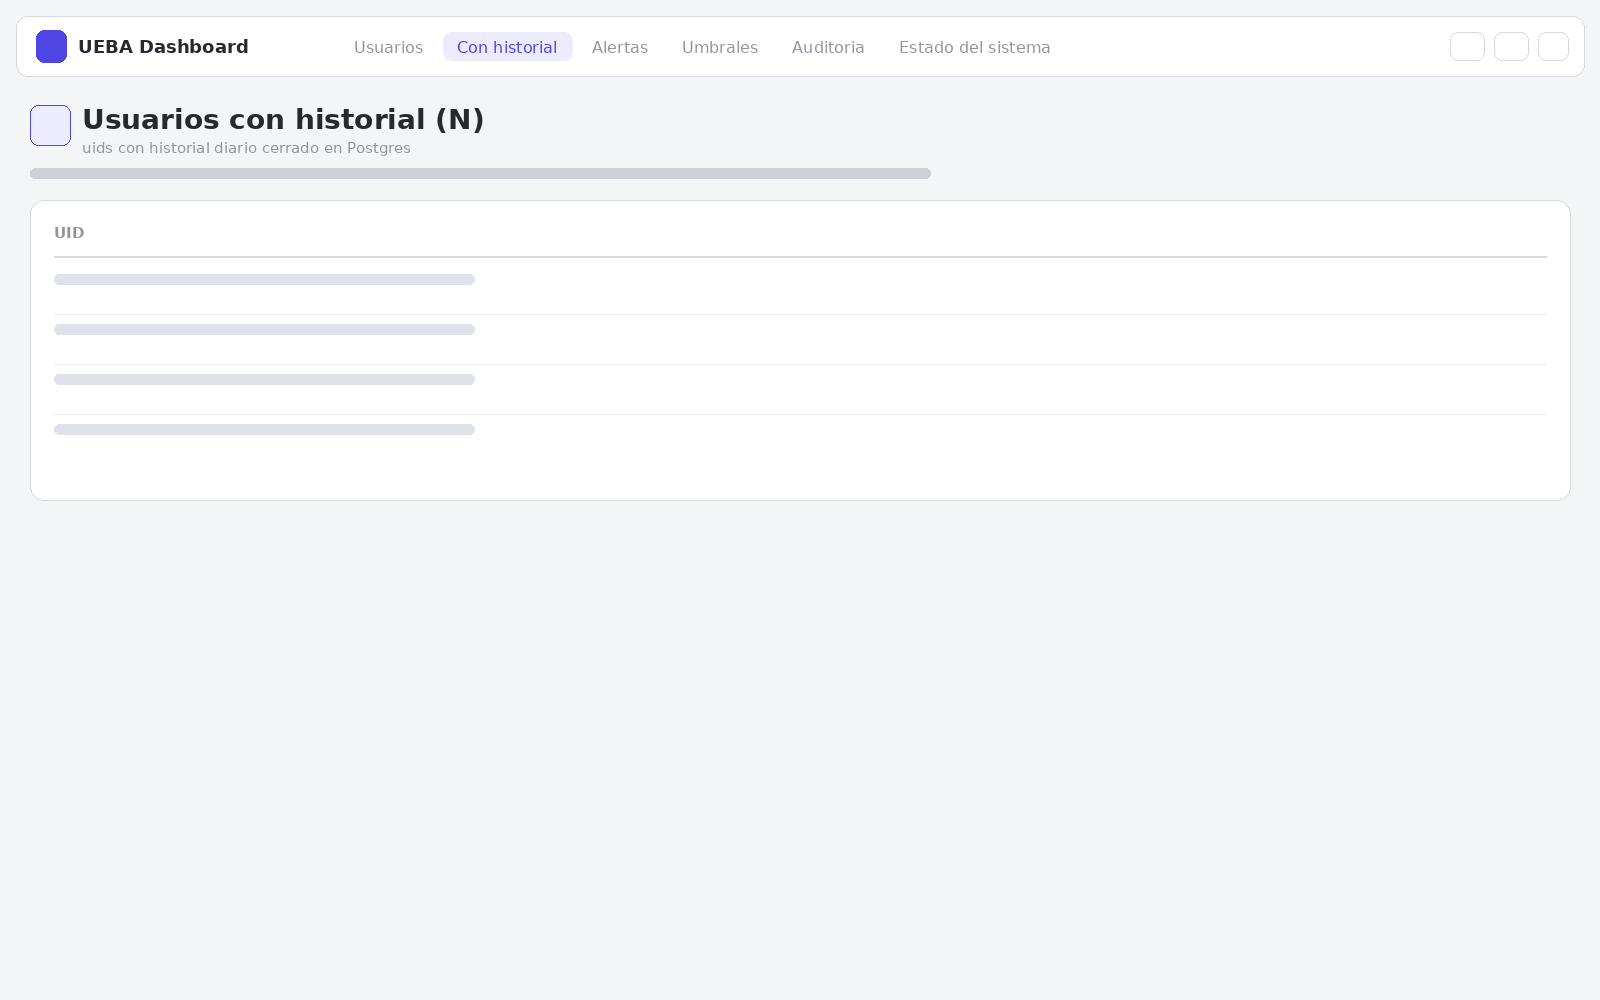
\includegraphics[width=0.8\textwidth]{images/mockups/mockup-historial-wireframe.png}
	\caption{Wireframe de baja fidelidad: Con historial}
	\label{fig:mockup-historial-wireframe}
	{\small Fuente: elaboración propia.\par}
	\bigskip
	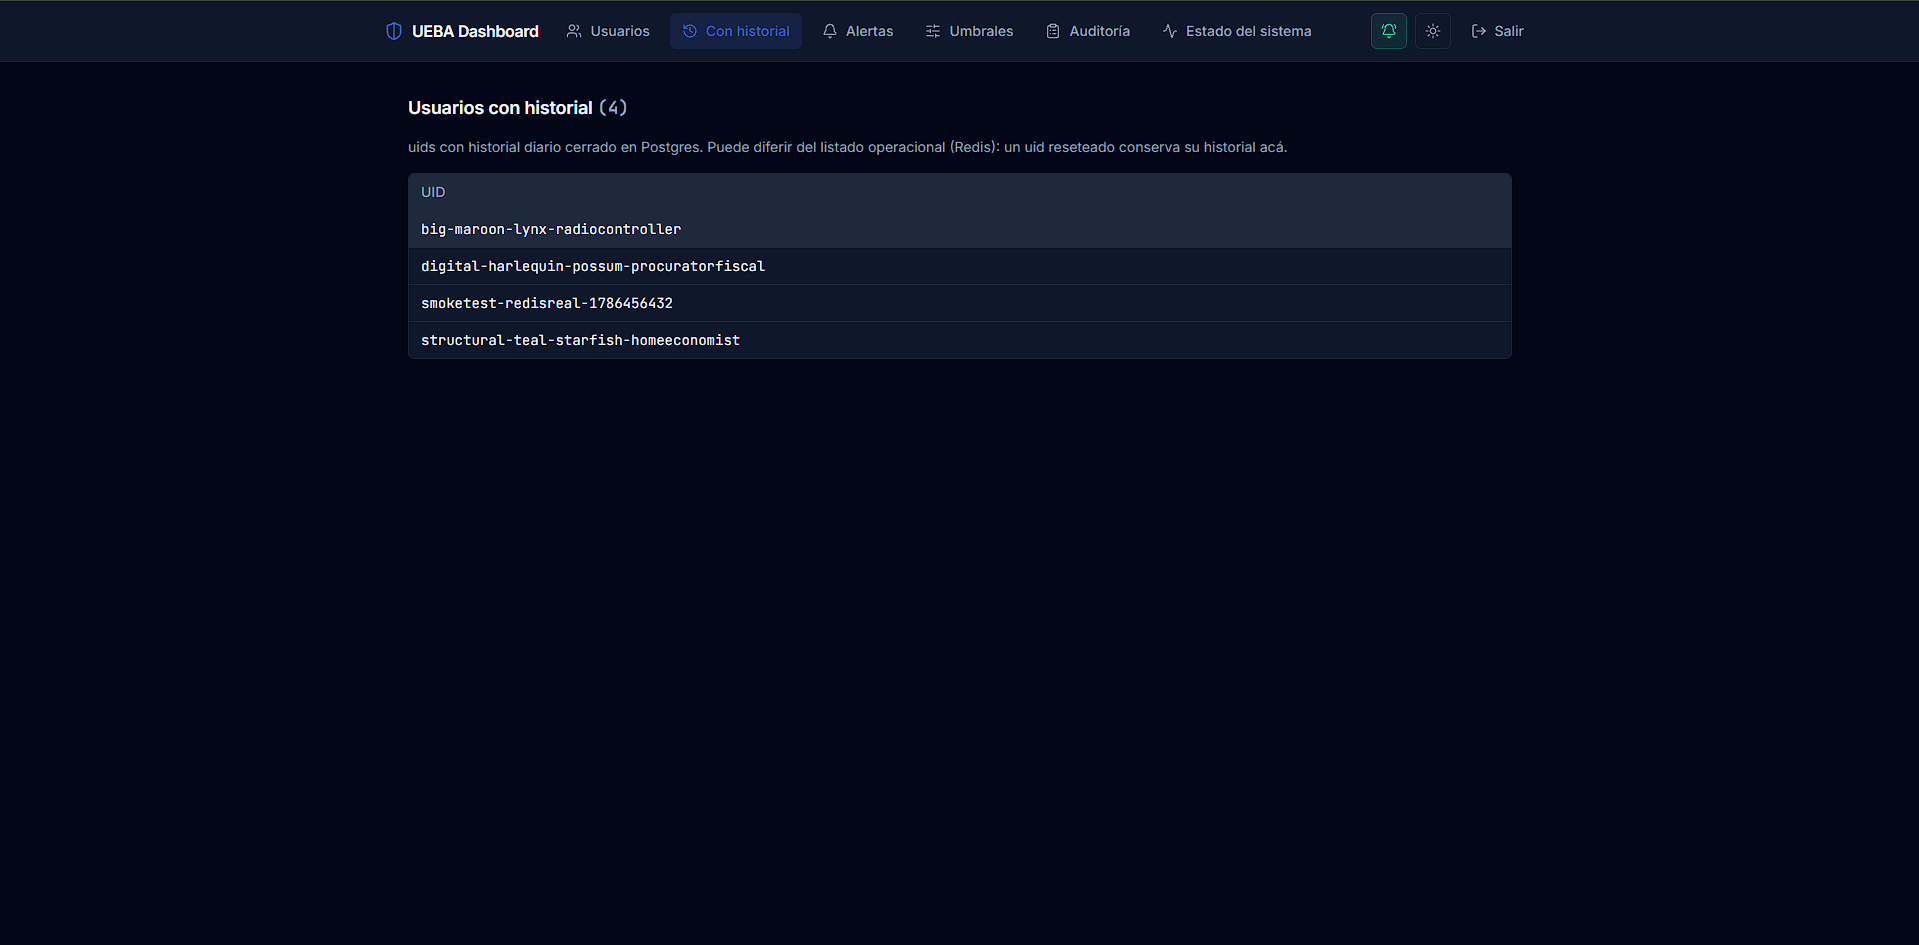
\includegraphics[width=0.8\textwidth]{images/mockups/mockup-historial-real.png}
	\caption{Pantalla real: \texttt{/historial}}
	\label{fig:mockup-historial-real}
	{\small Fuente: elaboración propia, captura del sistema.\par}
\end{figure}
\FloatBarrier

\begin{longtable}{p{1.8cm}p{12.8cm}}
	\caption{Justificación de diseño: Con historial}
	\label{tab:mockup-historial}\\
	\hline
	\textbf{ID} & \textbf{Justificación de diseño} \\
	\hline
	\endfirsthead
	\hline
	\textbf{ID} & \textbf{Justificación de diseño} \\
	\hline
	\endhead
	RF-16 (complementario) & Extiende la visibilidad en tiempo real del listado operacional con una vista de acceso a datos persistidos, sin mezclar ambas fuentes en una sola tabla. \\
	\hline
	Transparencia de diseño & La nota aclaratoria sobre la posible divergencia Redis/Postgres es una decisión de diseño explícita para que el administrador no interprete una ausencia en esta lista como ``sin historial real''. \\
	\hline
\end{longtable}
\FloatBarrier

\section{Decisiones de diseño transversales}
\label{sec:decisiones-transversales-mockups}
\begin{itemize}
	\item Tema oscuro por defecto (con alternancia a claro): reduce la fatiga visual en un panel pensado para monitoreo prolongado, y es el estándar de facto en herramientas de seguridad/observabilidad (SOC \emph{dashboards}) con las que el administrador ya está familiarizado.
	\item Codificación de color consistente por nivel de riesgo (bajo/medio/alto/crítico) en \emph{badges}, \emph{chips} de notificación y bordes de las tarjetas de umbral: la misma paleta se repite en Usuarios, Alertas y Umbrales, para que el administrador no tenga que reinterpretar el color en cada pantalla.
	\item Botones de guardado independientes por sección de formulario en vez de un único guardado global en \texttt{/umbrales}: reduce el riesgo de que el administrador modifique un umbral sin querer y termine también reescribiendo la configuración de notificaciones.
	\item Estados vacíos explícitos con mensaje (ej.\ ``Sin alertas activas'') en lugar de una tabla en blanco sin explicación, para que el administrador distinga un sistema sano de una posible falla de carga.
\end{itemize}

\clearpage
